\documentclass[a4paper, oneside, 12pt, bibliography = totocnumbered]{scrbook}

\usepackage[english, ngerman]{babel}
\usepackage[utf8]{inputenc}
\usepackage[xindy, nonumberlist, toc, numberedsection]{glossaries}
\usepackage[onehalfspacing]{setspace}

\usepackage{
	datetime,
	eurosym,
	float,
	graphicx,
	epstopdf,
	hyperref,
	listings,
	longtable,
	lscape,
	pdfpages,
	rotating,
	scrhack,
	tabu,
	wrapfig
}

\clubpenalty = 10000
\widowpenalty = 10000
\displaywidowpenalty = 10000

\hypersetup{
	colorlinks = true,
	linkcolor = black,
	urlcolor = black
}
		
\definecolor{backcolour}{rgb}{0.90, 0.90, 0.90}

\lstdefinestyle{default}{
	backgroundcolor = \color{backcolour},
	breaklines = true
	basicstyle = \tiny,
	columns = fullflexible
}

\renewcommand*{\glspostdescription}{}
\makeglossaries
\newacronym{gpio}{GPIO}{General Purpose Input/Output}
\newacronym{uart}{UART}{Universal Asynchronous Receiver Transmitter}
\newacronym{spi}{SPI}{Serial Peripheral Interface}
\newacronym{i2c}{I$^{2}$C}{Inter-Integrated Circuit}
\newacronym{pwm}{PWM}{Pulsbreitenmodulation (engl. Pulse Width Modulation)}
\newacronym{adc}{ADC}{Analog/Digital Converter}
\newacronym{soc}{SOC}{System on a Chip}
\newacronym{sbc}{SBC}{Single-Board Computer}
\newacronym{ftp}{FTP}{File Transfer Protocol}
\newacronym{aur}{AUR}{Arch User Repository}
\newacronym{tcp}{TCP}{Transmission Control Protocol}
\newacronym{css}{CSS}{Cascading Style Sheets}
\newacronym{html}{HTML}{Hypertext Markup Language}
\newacronym{dom}{DOM}{Document Object Model}
\newacronym{js}{JS}{JavaScript}
\newacronym{ssl}{SSL}{Secure Socket Layer}
\newacronym{json}{JSON}{JavaScript Object Notation}
\newacronym{http}{HTTP}{Hypertext Transfer Protocol}

\newglossaryentry{softwareRepository}{
    name = {Software Repository},
    description = {Versionsverwaltungssystem für Quellcode.}
}

\newglossaryentry{repository}{
    name = {Repository},
    plural = {Repositories},
    description = {Versionsverwaltungssystem.}
}

\newglossaryentry{ssl-offloading}{
    name = {SSL-Offloading},
    description = {Verfahren bei dem eingehende Pakete entschlüsselt werden und unverschlüsselt Netzintern weiterverschickt werden. Dadurch können nachgeschaltete Server entlastet werden.}
}

\newglossaryentry{capemgr}{
    name = {Capemgr},
    description = {Kernel-Mechanismus zum dynamischen Laden und Entladen von Device Tree Overlays.}
}

\newglossaryentry{devicetree}{
    name = {Device Tree},
    description = {Baumähnliche Datenstruktur zur Beschreibung von Hardware.}
}

\newglossaryentry{linux-distribution}{
    name = {Linux Distribution},
    plural = {Linux Distributionen},
    description = {Eine Sammlung von Programmen, die den Linux-Kernel als Betriebssystem und eine Anzahl von Anwendungen enthält. Dabei werden von verschiedenen Distributionen meist unterschiedlich Philosophien bezüglich Aktualität und Paketzusammenstellung verfolgt.}
}

\newglossaryentry{de-facto-standard}{
    name = {De-facto-Standard},
    description = {Ein etablierter aber nicht offiziell von einem Gremium verabschiedeter (technischer) Industriestandard.}
}

\newglossaryentry{digestAccessAuthentication}{
    name = {Digest Access Authentication},
    description = {Verfahren um Zugriffe auf Webserver-Verzeichnisse zu beschränken \cite{rfc7235}.}
}

\newglossaryentry{sameOriginPolicy}{
    name = {Same-Origin Policy},
    description = {Sicherheitsmechanismen für Webbrowser, die sicherstellen, dass HTML-Dokumente und Skripte immer Teil der eigentlichen Seite sind. Hierfür wird geprüft, ob der DNS-Name identisch ist \cite{zalewski2009}.}
}

\newglossaryentry{systemd}{
    name = {systemd},
    description = {Alternative Init-Prozesssteuerung; löst \textit{init} derzeit in vielen Distributionen ab.}
}

\newglossaryentry{init}{
    name = {init},
    description = {Initialisierungsprozess unter Linux.}
}

\lstset{style = default}

\bibliographystyle{unsrtdin}

\author{Caspar Friedrich}
\title{Webgestütztes GPIO Management am Beispiel des BeagleBone Black}

\begin{document}

%Titlepages
% Deutsche Titelseite
\begin{titlepage}
\begin{center}

% FH-Logo

\includegraphics[width = \textwidth]{images/imp_rechts.eps}\\[3cm]

% BA + Thema
Bachelorarbeit Medientechnik\\[0.5cm]
{\sffamily \bfseries \Huge Webgestütztes GPIO Management\\[0.25cm]
am Beispiel des BeagleBone Black}\\[2cm]

% Info Student
vorgelegt von\\[0.5cm]
\textbf{Caspar Friedrich}\\[0.5cm]
Mat.-Nr. 11062078\\[0.5cm]

\vfill

% Unterer Teil der Seite
Erstgutachter: Prof. Dr. Klaus Ruelberg (Fachhochschule Köln)\\[0.5cm]
Zweitgutachter: Prof. Dr. Luigi Lo Iacono (Fachhochschule Köln)\\[0.5cm]
Dezember 2014

\end{center}
\end{titlepage}
\begin{otherlanguage}{english}

\begin{titlepage}
\begin{center}

% FH-Logo

\includegraphics[width = \textwidth]{images/imp_rechts.eps}\\[3cm]

% BA + Thema
Bachelor Thesis\\[0.5cm]
{\sffamily \bfseries \Huge Webbased GPIO Management using\\[0.25cm]
the example of the BeagleBone Black}\\[2cm]

% Info Student
submitted by\\[0.5cm]
\textbf{Caspar Friedrich}\\[0.5cm]
Mat.-Nr. 11062078\\[0.5cm]

\vfill

% Unterer Teil der Seite
First Reviewer: Prof. Dr. Klaus Ruelberg (Fachhochschule Köln)\\[0.5cm]
Second Reviewer: Prof. Dr. Luigi Lo Iacono (Fachhochschule Köln)\\[0.5cm]
\monthname ~\the\year

\end{center}
\end{titlepage}

\end{otherlanguage}

%Overview
% Uebersichtsseite, deutscher Abschnitt
\begin{center}
	\textbf{Bachelorarbeit}
\end{center}

\noindent \textbf{Titel:} Webgestütztes GPIO Management am Beispiel des BeagleBone Black\\

\noindent \textbf{Gutachter:}
\begin{itemize}
	\item Prof. Dr. Klaus Ruelberg (Fachhochschule Köln)
	\item Prof. Dr. Luigi Lo Iacono (Fachhochschule Köln)
\end{itemize}

\noindent \textbf{Zusammenfassung:} In der vorliegenden Bachelorarbeit wird ein netztwerk-gestütztes Messsystem vorgestellt, das mit Hilfe verschiedener GPIO des BeagleBone Black eine entfernte Messstationen ermöglicht. Die Besonderheit des Systems liegt darin, dass es als Basis ohne irgendeine Anwendungs-Spezialisierung besteht – also flexibel einsetzbar ist und gleichzeitig im Verhältnis zu heute gängigen Messsystemen sehr kostengünstig.  Es ist einfach und vielseitig konfigurierbar und kann browserbasiert über ein Netzwerk gesteuert und überwacht werden.\\

\noindent \textbf{Stichwörter:} BeagleBone, Webinterface\\

\noindent \textbf{Datum:} {\longdate \today}
\newpage
% Uebersichtsseite, englischer Abschnitt
\begin{otherlanguage}{english}

\begin{center}
	\textbf{Bachelor Thesis}
\end{center}

\noindent \textbf{Titel:} Webbased GPIO Management using the example of the BeagleBone Black\\

\noindent \textbf{Reviewers:}
\begin{itemize}
	\item Prof. Dr. Klaus Ruelberg (Cologne University of Applied Sciences)
	\item Prof. Dr. Luigi Lo Iacono (Cologne University of Applied Sciences)
\end{itemize}

\noindent \textbf{Abstract:} In this Bachelor Thesis I present a net-supported measuring system which provides a remote measuring station by help of the BeagleBone Black GPIOs. The outstanding feature of this system is its basic configuration, that has no defined use case and thus allows a flexible implementation in various measurement situations. Consequently, the system is economical and easyly applicable in almost any laboratory situation.\\

\noindent \textbf{Keywords:} BeagleBone, Webinterface\\

\noindent \textbf{Date:} {\longdate \today}

\end{otherlanguage}
\newpage

\tableofcontents

\part{Dokumentation}
\chapter{Einleitung}

\glqq We have a clear vision – to create a world where every object - from jumbo jets to sewing needles – is linked to the Internet.\grqq \cite[Helen Duce, Seite 1]{iot2020}

Das \textit{Internet of Things} ist ein rasant wachsender Anwendungsbereich. Angetrieben von einer zunehmenden Akzeptanz digitaler Systeme und der günstigen Entwicklung von Baugröße, Leistung und Zuverlässigkeit und nicht zuletzt der sinkende Preis haben dazu geführt, dass digitale Systeme heute in allen Lebensbereichen anzutreffen sind \cite{iot2020, weiser1991}.\\

Es ist inzwischen selbstverständlich, Steuerungssysteme in der Industrie, zum Teil sogar schon im privaten Haushalt, miteinander zu vernetzen und im Netzwerk zugänglich zu machen. So ist es möglich, die vorhandenen Daten jederzeit auch extern z. B. via Mobiltelefon abzurufen. Heute sind viele Geräte und Programme sehr spezialisiert, so dass man in komplexen Arbeitszusammenhängen viele verschiedene Systeme braucht. Dadurch ist oft auch ein hoher finanzieller Aufwand erforderlich.

Gleichzeitig hat eine Annäherung der Hardwarehersteller an die \glqq Hobby\grqq -Entwickler stattgefunden und Projekte wie Arduino und Co. haben den Entwicklungsaufwand eigener Hard- und Software erheblich reduziert. Damit wird es erheblich erleichtert, bei individuellen Fragestellungen selber individuelle Lösungen zu entwickeln. Hat man nun viele individuelle Lösungen gefunden und somit viele verschiedenartige Messdaten erhalten, besteht die Notwendigkeit, diese wiederum zusammenzuführen.


\section{Zielsetzung}
Aus dieser Tendenz entstand die Idee, die unterschiedlichen im Laboralltag anfallenden Messungen mit einem einzigen flexiblen System zu steuern und die Resultate gemeinsam verfügbar zu machen. 

Ziel dieser Arbeit ist es, ein Steuersystem für Messanwendungen zu entwickeln, das sich einfach konfigurieren lässt, flexibel in der Anwendung ist und gleichzeitig kostengünstig bleibt. Besonderes Augenmerk soll dabei auf der ausreichenden Verfügbarkeit verschiedener \gls{gpio} liegen. Insbesondere Pulsbreitenmodulation und Analog/Digital-Konverter sind für Messanwendungen interessant. Die anfallenden Messdaten sollen protokolliert werden und extern verwendbar sein. Die zu entwickelnde Applikation soll auf keinen bestimmten Anwendungsfall spezialisiert sein. Sie soll vielmehr dem Anwender die Möglichkeit geben, sich eine für sein jeweiliges Projekt passende Umgebung zusammenzustellen. Weiter soll das System ohne ständige Überwachung arbeiten können. Es soll möglich sein, eine  entfernte Messstation aufzubauen, die nach Belieben via LAN, WLAN oder auch GSM konfiguriert und überwacht werden kann.\\

\vfill

\includegraphics[width = \textwidth]{images/Einleitung.eps}

\vfill

\section{Definitionen}
In dieser Arbeit wird ein Singleboard-Computer des Typs \textbf{BeagleBone Black Rev. A5C} verwendet. Andere Versionen dieses Computers sind, sofern kompatibel, ebenfalls verwendbar, allerdings nicht getestet. Um eine gute Lesabrkeit zu ermöglichen, ist mit \glqq BeagleBone\grqq ~im Folgenden immer diese Version gemeint.
\chapter{Grundlagen}

\section{Hardware}

\subsection{\glsentrylong{sbc}}
Ein \gls{sbc}, zu deutsch Einplatinenrechner, ist ein Computersystem, bei dem alle für die Verwendung nötigen Bauteile auf einer einzelnen Platine aufgebracht sind. Hierbei sind neben den essenziellen Komponenten wie Prozessor, RAM und ROM auch Controller für verschiedene I/O-Schnittstellen, Oszillatoren oder Co-Prozessoren verbaut. Single-Board Computer werden vor allem in der Industrie als Steuersysteme eingesetzt, da sie oft billiger und flexibler sind als fest verdrahtete Steuersysteme. Mit fortschreitender Miniaturisierung und steigender Leistungsfähigkeit finden SBC's heute auch in alltäglichen Geräten wie Autos, Waschmaschienen oder auch Fernbedienungen Verwendung.\\

Technisch gesehen sind auch erste Heimcomputer wie der \emph{C64} oder \emph{Atari ST} Single-Board Computer, allerdings lassen sich diese ohne Ein- und Ausgeabegräte wie Maus, Tastatur, Bildschirm nicht sinnvoll nutzen und werden in der Regel nicht als solche bezeichnet.


\subsubsection{Schnittstellen}
Single-Board Computer verfügen, je nach Anwendungsgebiet, über eine Vielzahl verschiedener analoger und digitaler I/O-Schnittstellen.\\

\noindent Übliche Schnittstellen sind:

\begin{itemize}
  \item \gls{gpio}, darunter digitale I/O, \gls{pwm} und \gls{adc}
  \item \gls{uart}
  \item \gls{spi}
  \item \gls{i2c}
\end{itemize}

Über \gls{uart} isteine Implementierung der verbreiteten RS232/422/485-Schnittstellen möglich und auch üblich.\\

Aktuelle (Entwickler-)Systeme haben in der Regel einen oder mehrere USB-Anschlüsse (sowohl Client als auch Host Ports sind üblich) oder zumindest einen JTAG-Port, was die Programmierung wesentlich vereinfacht. In der Regel verfügen leistungsstärkere Systeme auch über einen Grafikausgang, Oft HDMI oder eine der Miniaturvarianten.


\subsection{\glsentrylong{soc}}
Eng verknüpft mit der Entwicklung der SBC ist das Konzept des \gls{soc}. Hierbei werden die meisten oben genannten Komponenten eines Systems direkt in einem einzelnen IC verbaut. Meist sind nur ROM und Controller für höhere Schnittstellen USB oder LAN (in manchen Fällen auch Grafik) extern angebunden.

Heutige Single-Board Computer mit einem SOC können sehr leistungsstark sein, sind als Mehrkernsystem aufgebaut und haben Taktraten von mehreren GHz. Diese Computer sind vom Design her stark an Desktop-Systeme angepasst und können mit einem vollwertigen Linux- oder Windows-System betrieben werden.

Gerade bei diesen leistungsstarken SOCs hat sich die ARM-Architektur durchgesetzt. 1983 als Nebenprojekt gegründet hatte die 32-Bit-Architektur bereits 2002 einen Marktanteil von fast 80\% \cite{stiller2002}.\\

\noindent \gls{sbc} lassen sich (sehr) grob in zwei Klassen unterteilen:

\begin{enumerate}
\item \textbf{Leistungsschwache Systeme}\\
Die Taktraten dieser Prozessoren liegen üblicherweise deutlich unter 50MHz, in seltenen Fällen bis 100MHz. Diese Mikrocontroller werden meist direkt programmiert und finden vor allem im low energy-Sektor Anwendung.
\item \textbf{Leistungsstarke Systeme}\\
Hier ligen die Taktraten meist im GHz-Bereich. Hauptanwendungsbereiche sind Mobilfunksysteme und embedded computing in der Industrie. Gerade im Mobilfunkbereich sind oft Mehrkernsysteme anzutreffen und es wird bis auf wenige Ausnahmen oberhalb eines Betriebssystems, meist Linux bzw. Android, programmiert.
\end{enumerate}


\subsection{BeagleBone Black}
Für diese Arbeit verwende ich einen BeagleBone Black Rev. A5C (im Folgenden BeagleBone), ein Entwickler-Board mit einem ARM\textregistered ~Cortex\texttrademark -A8 Prozessor (Single Core) von Texas Instruments.\\

\noindent Die wichtigsten Features:
\begin{itemize}
  \item 1GHz Taktrate
  \item 512MB DDR3 RAM
  \item 2GB\footnote{4GB ab Rev. C} Onboard Flash Memory
  \item 10/100 Mbit/s Ethernet
  \item 69\footnote{27 GPIO sind ohne weitere Konfiguration direkt verfügbar} \gls{gpio} mit mehreren \gls{pwm}-Ausgängen und \gls{adc}-Eingängen
  \item Verhältnismäßig geringer Preis von ca. \EUR{45}
\end{itemize}


\section{Betriebsysteme}
Da die Ressourcen des BeagleBone Black sehr begrenzt sind, wird für diese Arbeit ein schlankes Betriebssystem benötigt, welches nur wenig Speicher verbraucht und geringen Leistungs-Overhead verursacht. Für diesen Zweck gibt es spezielle Versionen der bekannten Betriebssysteme wie Microsoft Windows oder Linux sowie verschiedene \glqq unixoide\grqq ~Betriebssysteme.


\subsection{Linux}
Linux hat den Vorteil, dass nahzu alle Software als Quellcode verfügbar ist und im Zweifel angepasst werden kann. Zudem ist es üblich Lizenzen zu verwenden, die eine nicht-kommerzielle Anwendung sowie Anpassungen kostenfrei zulassen.

Ein eigenes Linux zu entwickeln oder ein Build System\footnote{Einige Distributionen verwenden ein sog. Build System, bei dem die benötigten Kernelmodule und Softwarepakete selbst zusammengestellt werden können.} zu verwenden wäre aus Sicht der Performance sicherlich die beste Wahl und ist in der Industrie weitgehend üblich. Das würde allerdings den Rahmen dieser Arbeit sprengen. Zudem gibt es einige sehr schlanke und bereits für den BeagleBone angepasste \glspl{linux-distribution}.


\subsection{Linux Distributionen}
\href{http://beagleboard.org/}{BeagleBoard.org} bietet für den BeagleBone Black zwei verschiedene Distributionen an: {\AA}ngström und Debian. Beide Distributionen haben Vor- und Nachteile, die weier unten erlätert werden. Ein weiteres Projekt, welches sich unter Entwicklern großer Beliebtheit erfreut ist Arch Linux, das als Basis für diese Anwendung dienen soll.

\subsubsection{The {\AA}ngström Distribution}
The {\AA}ngström Distribution ist auf dem BeagleBone vorinstalliert und stellt die Hauptdistribution dar. Diese Distribution nutzt ein Build System und findet im Wesentlichen Anwendung bei Speichersystemen wie NAS oder FTP-server, wichtigstes Feature ist daher der geringe Leistungs- und Speicherbedarf. Bei dieser Distribution muss allerdings nahezu jede nicht-standard Software selbst kompiliert und eingerichtet werden.

\subsubsection{Debian Linux}
Im Allgemeinen gilt Debian Linux als (rock-)stable und ist eine der verbreitetsten Distributionen. Zudem basieren einige weitere namhafte Distributionen auf Debian Linux. Stärke und gleichzeitig auch Schwäche dieser Distribution sind die langen und umfangreichen Softwaretests. Wenn ein Paket in den offiziellen Repositories verfügbar ist kann man zwar davon ausgehen, dass es fehlerfrei funktioniert und mit allen anderen angebotenen Paketen kompatibel ist. Allerdings liegt es meist nicht mehr in der aktuellen Version vor. Das kann gerade bei Software aus dem Bereich Netzwerk/Internet problematisch werden.

\subsubsection{Arch Linux}
Gegenüber den oben genannten Distributionen hat Arch Linux zwei wesentliche Vorteile: Zum einen gibt es eine (Sub-)Distribution speziell für ARM-Prozessoren, bei der das Basissystem mit ca. 500MB sehr schlank ist. Zum anderen stellt Arch Linux ARM ein sehr umfangreiches \gls{softwareRepository} mit hoher Aktualität zur Verfügung. Zusätzlich gibt es das \gls{aur}, ein freies \gls{repository} in dem jeder Nutzer seine Pakete einstellen kann. Sämtliche in diesem Projekt verwendete Software lässt sich entweder direkt via Paketverwantung aus den offiziellen \glspl{repository} installieren oder kann vom Anwender selber kompiliert werden.

Arch Linux ARM verwendet ein Rolling-Release-Konzept, ein System kontinuierlicher Software-Entwicklung, bei der Pakete separat aktuell gehalten und weiter entwickelt werden. Es gibt keine explizite Betriebssystemversion sondern sog. Snapshots. So ist es  wesentlich einfacher, das System aktuell und sicher zu halten. Zwar kann es durchaus passieren, dass die eingestellte Software nicht out-of-the-box funktioniert. Aber in der sehr aktiven Community hinter Arch Linux bekommt man relativ schnell Hilfe.

Die Kernel-Entwicklung schreitet derzeit sehr schnell voran, daher wird zusätzlich zur regulären Kernel-Entwicklung  ein Legacy-Paket mit einer stabilen Version (3.8) gepflegt, um nach einem Update des Kernelpaketes nicht erst die Kompatibilität wieder herstellen zu müssen.


\section{Webtechnologien}
In dieser Arbeit kommen eine Vielzahl unterschiedlicher Webtechnologien zum Einsatz. An dieser Stelle alle zur Verfügung stehenden Technologien im Detail zu beschreiben, würden den Rahmen der Arbeit sprengen. Ich beschränke mich hier darauf, die Architektur des Projektes zu darzustellen. Meine Auswahl an Software erläutere ich im Zusammenhang in Kapitel 4: Implementierung.

\subsection{Webserver}
Als Webserver wird in der Regel eine Software bezeichnet, die verschiedene Dokumente an einen Client, z. B. ein Webbrowser, ausliefert. Oft wird auch die ganze Hardware, auf der ein Webserver betrieben wird, als Webserver bezeichnet. Dies ist dann der Fall, wenn der Rechner ausschließlich zu diesem Zweck betrieben wird, z. B. bei größeren Webseiten.

Auf Grund verschiedener Spezialisierungen und Ansätze gibt es heute eine große Anzahl verschiedener Webserver. Apache HTTP Server der gleichnamigen Firma und Microsofts IIS haben sich hier in den letzten Jahren deutlich von der Konkurenz absetzen können. \cite{webserversurvey1014}. IIS kommt für diese Arbeit allerdings nicht in Frage, da er nicht für Linux angeboten wird.

\subsubsection{Lighttpd}
Lighttpd ist ein Webserver, der durch seine besonders ressourcenschonende Implementierung hervorsticht. Dieser Webserver ist darauf spezialisiert, statische Dokumente auszuliefern, was ihn besonders passend für diese Arbeit macht. Außerdem lässt er sich wesentlich einfacher konfigurieren und über Module erweitern als andere weiter verbreitete Webserver \cite{krieg2009}.


\subsection{Node.js}
\label{subsec:Node.js}
Node.js ist ein JavaScript-Framwork, das auf Googles V8-JavaScript-Engine basiert. Es stellt eine serverseitige Umgebung zur Verfügung, über die sich komplexe Netzwerkanwendungen leicht programmieren lassen. Dabei stellt Node.js ein Modulkonzept vor, mit man relativ unkompliziert Programmteile auslagern oder weitere Funktionalität einbinden kann. In der Basisinstallation liefert Node.js bereits eine große Bandbreite an Modulen mit, sodass viele Anwendungen ohne zusätzliche Software umgesetzt werden können \cite{springer2013}.

\subsubsection{npm}
Der Node Package Manager (NPM) erweitert Node.js um ein Werkzeug, mit dem sich externe Module leicht herunterladen und einbinden lassen. Unter \href{https://www.npmjs.org/}{npmjs.org} können zudem weitere Informationen und in der Regel auch eine API der Module eingesehen werden. Dank einer großen Community lassen sich hier zu den meisten allgemeinen Problemen bereits einige Lösungsansätze finden.

\subsubsection{bonescript}
Ausschlaggebend für die Verwendung von Node.js ist das Modul \textit{bonescript} von Jason Kridner, Mitgründer der \href{http://beagleboard.org/}{BeagleBoard.org} Foundation. Dieses Modul steuert über eine übersichtliche API weite Teile der Hardware, sodass auch hier der Arbeitsaufwand deutlich verringert wird.

\subsection{WebSockets}
WebSockets stellen eine Möglichkeit dar, Daten zwischen Client, z. B. der Browser und Server auszutauschen. Wie auch \gls{http} basieren WebSockets auf \gls{tcp}, sind dabei aber wesendtlich schneller. Im Gegensatz zu \gls{http} ist über WebSockets eine Vollduplex-Verbindung möglich. Die Metadaten sind zudem überschaubar, sodass hierbei wenig zusätzliche Netzwerklast entsteht. Ein weiterer Vorteil ist, dass WebSockets von der \gls{sameOriginPolicy} ausgeschlossen sind \cite{rfc6455}.
\chapter{Konfiguration des Betriebssystems}

Ein essentieller Punkt zu Beginn des Projektes ist die Auswahl des Betriebssystems, da im weiteren Verlauf alle Entwicklungen darauf aufbauen werden. Außerdem ist ein Teilziel des Projektes, schon existierende Software zu nutzen, um den Entwicklungsaufwand klein zu halten und den Fokus auf die eigentliche Fragestellung zu richten. Also habe ich das bereits auf dem BeagleBone vorinstallierte Betriebssystem - {\AA}ngström Linux - intensiv getestet.\\

\noindent Die grundlegenden Fragen waren:

\begin{itemize}
  \item Gibt es genügend Speicherplatz für die zu entwickelnde Software?\\
  Wie schaffe ich bei Bedarf weiteren Speicherplatz für meine Anwendungen?
  \item Wird die zusätzlich gebrauchte Software (Webserver, FTP-Server, etc...) in einem Repository zur Verfügung gestellt?
  \item Sind ausreichend Rechenleistung und Arbeitsspeicher verfügbar, um zusätzliche Dienste zu betreiben?
  \item Sind die benötigten Systemressourcen (Netzwerkports u.a.) verfügbar, bzw. kann ich sie ohne großen Aufwand freigeben?
\end{itemize}

Die Tests ergaben, dass das Betriebssystem mit einer graphischen Oberfläche und mehreren Netzwerkdiensten ausgeliefert wird. 
Die graphische Oberfläche verbraucht Systemressourcen und Speicherplatz, ist aber überflüssig, da das System headless betrieben werden soll. Dazu laufen ein Apache Webserver, eine Cloud9 Entwicklungsumgebung und ein Websocket Server. Des weiteren verwendet {\AA}ngström Distribution parallel zwei verschiedene Daemon Manager (\gls{systemd} und \gls{sysvinit}). Diese erschweren das Arbeiten mit {\AA}ngström Linux erheblich.

Die Software, die ich für mein Projekt verwenden möchte, liegt nicht in den offiziellen Repositories vor. Also müßte ich sie selber konfigurieren und kompilieren.

Aus diesen Erfahrungen folgt, dass {\AA}ngström Linux nicht das richtige Betriebssystem für mein Projekt ist. Der Aufwand, es an meine Bedürfnisse anzupassen, wäre größer als auf eine andere Distribution zurückzugreifen.\\

Die zweite vom Hersteller des BeagleBone angebotene Distribution ist Debian Linux. Auch diese habe ich nach den oben genannten Kriterien geprüft. Die Konfiguration, die schon zum Ausschluss von {\AA}ngströn Linux führte, fanden sich im Prinzip auch hier. Auf \href{http://www.armhf.com/}{ARMhf.com} gibt es zwar eine weitere Debian-Installation bereits fertig als Linux Image. Diese hat nicht die oben erwähnten Eigenheiten, nutzt aber die neueste Kernel-Version, die mit der Bonescript Library nicht kompatibel ist. Ein Kernel-Downgrade wäre möglich, ist aber grundsätzlich und unter Debian im Besonderen sehr aufwändig. Daher eignet sich Debian Linux ebenfalls nicht für mein Projekt.\\

Eine weitere Distribution für BeagleBone ist Arch Linux. Die Besonderheit dieser Distribution ist, dass die Basisinstallation sehr Ressourcen schonend ist. Sie enthält keinerlei Software, die nicht für den grundsätzlichen Betrieb erforderlich ist. Gleichzeitig stellt sie Werkzeuge zur Verfügung, um die benötigte Software bequem aus umfangreichen Repositories zu installieren. Abweichend von der regulären Kernel-Entwicklung wird die hier benötigte Kernel-Version (3.8) und entsprechende Header Files über die Pakete \textit{linux-am33x-legacy} und \textit{linux-headers-am33x-legacy} bereitgestellt.\\

Somit ist meines Erachtens Arch Linux das richtige Betriebssystem für dieses Projekt. Darüber hinaus kenne ich es seit langem, da ich es beruflich wie privat auf Desktop Computern verwende. Ich muss mich also nicht in eine neue Distribution einarbeiten.


\section{Software}

Zusätzlich zu den mitgelieferten Pakteten der Distribution werden noch einige zusätzliche Pakete benötigt, die aber keiner besonderen Konfiguration benötigen und daher hier nicht näher erklärt sind. In Tabelle \ref{tab:additionalPackages} findet sich eine Liste mit diesen Paketen.\\

Desweiteren werden ein HTTP-Server und die JavaScript Engine für den WebSocket Server benötigt. Der Proxy-Server sorgt dafür, dass die Seite von außen über einen einzigen Port erreichbar ist und dass mit geringem Aufwand \gls{ssl}-verschlüsselte Verbindungen hergestellt werden können. Zusätzlich wird noch ein FTP-Server installiert, um Messdaten ohne Webinterface abrufen zu können (Abb. \ref{fig:componentsServer}).

\begin{figure}[ht]
  \centering
  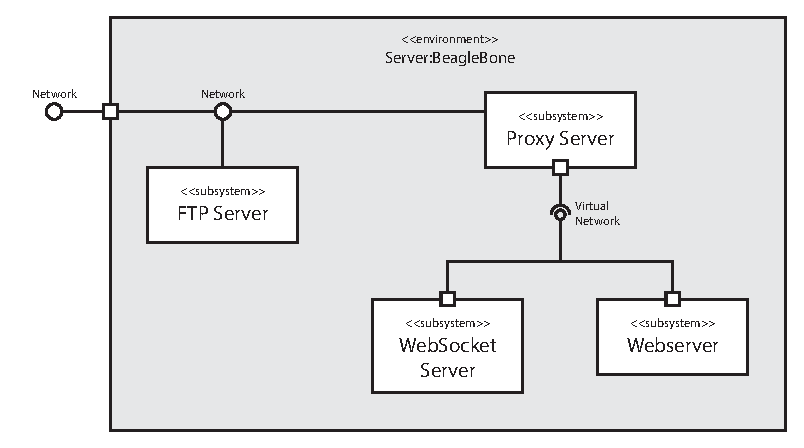
\includegraphics[width = 0.8\textwidth]{documentation/images/componentsServer.eps}
  \caption{Komponenten des boneserver}
  \label{fig:componentsServer}
\end{figure}


\subsection{Proxy Server -- HAProxy}
\label{subsec:HAProxy}
HAProxy ist ein Proxy-Server, der eigentlich eingesetzt wird, um Anfragen via \gls{tcp} auf mehrere Server zu verteilen. Wesentlich interessanter für diese Arbeit ist allerdings, dass der HAProxy, ab Version 1.5, sog. \gls{ssl-offloading} unterstützt und nativ \gls{ssl}-verschlüsselte Verbindungen verarbeiten kann. Dabei erfüllt bereits eine einfache Basis-Konfiguration bereits diese Aufgabe \cite{kuehnast2014}.

In diesem Projekt wird HAProxy eingesetzt, um WebSocket Requests von regulären HTTP Requests zu trennen und auf unterschiedliche Dienste weiterzuleiten. Ziel dieser Maßnahme ist es, nach außen die gesamte Website hinter einem Port zu betreiben, obwohl die beiden Prozessen völlig von einander getrennt sind. So ist die Gefahr minimal, dass bei einem Feldeinsatz der Port für den WebSocket Server von einer Firewall blockiert wird. Die Website ist somit entweder vollständig erreichbar oder gar nicht. Auch ist der WebSocket Server, der systembedingt mit root-Rechten laufen muss, ausschließlich per WebSocket über den Proxy-Server zu erreichen und so gegenüber Angriffen von außen weitgehend sicher.

Ein weiterer wichtiger Punkt ist, dass sich für jeden Server die maximale Anzahl der aktiven Verbindungen bequem per Konfigurationsdatei einstellen lassen. So wird ohne besondere Programmierung sichergestellt, dass immer nur eine Verbindung zum WebSocket Server besteht. Alle weiteren Verbindungsanfragen werden auf eine Warteliste gesetzt und weitergeleitet, sobald der Websocket Server wieder frei wird.\\

Die Konfigurationsdatei findet sich im Repository unter \textit{config/haproxy/haproxy.cfg} und wird bei der Installation automatisch verlinkt.
Hervorgehoben werden sollen zwei Parameter:

\begin{lstlisting}
maxconn 1
\end{lstlisting}
weist HAProxy an, wie oben beschrieben, nur eine aktive Verbindung zu diesem Server zuzulassen.

\begin{lstlisting}
ssl crt /opt/boneserver/config/haproxy/testcert.crt
\end{lstlisting}
macht das Einbinden eines \gls{ssl}-Zertifikates möglich. Nach der Installation ist hier ein Testzertifikat eingetragen um, \gls{ssl}-Verbindungen zumindest technisch testen zu können.


\subsection{Webserver -- Lighttpd}
\label{subsec:Lighttpd}
Lighttpd wird in dieser Arbeit verwendet, um statische HTML-Dokumente und JavaScript-Dokumente auszuliefern und die Software vor nicht autorisierten Zugriffen zu schützen. Die Konfigurationsdatei findet sich unter \textit{config/lighttpd/lighttpd.conf}.\\

Abweichend von der üblichen Verwendung eines Webservers sind einige Parameter hervorzuheben.

\begin{figure}[ht]
  \begin{lstlisting}
  server.bind = "localhost"
  server.port = 8080
  \end{lstlisting}
  \caption{Lighttpd ist nur lokal über Port 8080 erreichbar}
  \label{lst:lighttpdLocal}
\end{figure}

Abbildung \ref{lst:lighttpdLocal} zeigt, dass der Webserver ausschließlich lokal erreichbar ist. Weiter darf Lighttpd nicht an Port 80 arbeiten, um Konflikte mit HAProxy zu vermeiden.\\

\begin{figure}[ht]
  \begin{lstlisting}
  auth.backend = "htdigest"
  auth.backend.htdigest.userfile = "/etc/lighttpd/lighttpd.user"
  auth.require = (
    "/" => (
      "method" => "basic",
      "realm" => "Administrators",
      "require" => "valid-user"
    )
  )
  \end{lstlisting}
  \caption{Digest Access Authentication-Konfiguration}
  \label{lst:lighttpdhtdigest}
\end{figure}

In Abbildung \ref{lst:lighttpdhtdigest} wird beschrieben, wie der Zugriff auf einzelne Verzeichnisse via \gls{digestAccessAuthentication} beschränkt wird. So wird sichergestellt, dass der boneserver nur von autorisierten Nutzern gesteuert werden kann.

Jeder \textit{auth.require}-Block stellt eine Zugriffsregelung dar. User werden in der Datei \textit{lighttpd.user} eingetragen, diese Einträge können bequem über diverse Online-Generatoren erstellt werden. Das hat den Vorteil, dass bei einer eventuellen Weiterentwicklung der Software neue User und auch weitere Zugriffsebenen implementiert werden können. Das dafür benötigte Modul ist \textit{mod\_auth} und wird unter \textit{server.modules} eingetragen.


\subsection{FTP-Server -- vsftpd}
\label{subsec:vsftpd}
Um die Verwendung in einer weitgehend automatisierten Umgebung zu ermöglichen, ist vsftpd als FTP\footnote{File Transfer Protocoll}-Server installiert. Messdaten können dann auch per FTP abgerunfen und verwaltet werden. Neben den üblichen Einstellungen wird über die beiden Parameter

\begin{lstlisting}
local_enable=YES
anonymous_enable=NO
\end{lstlisting}
sichergestellt, dass auch hier nur autorisierte Nutzer Zugriff haben. Hierbei verwendet vsftpd die lokalen Nutzerkonten, in diesem nur das root-Konto, zur Authentifikation. Vsftpd lässt sich dabei leicht dahingehend erweitern, dass auch zusätzliche Nutzer mit spezifischen Zugriffsrechten eingerichtet werden können.


\subsection{JavaScript Engine -- Node.js}

Zusätzlich zu den bereits enthaltenen Modulen werden noch drei Module benötigt, um einen WebSocket Server zur Verfügung zu stellen und die Steuerung der GPIO zu realisieren. Die Module selbst bedürfen keiner weiteren Konfiguration.

\begin{longtabu} to \textwidth {
  X[1]
  X[5]}
  \textbf{bonescript} & Dieses Modul übernimmt die Steuerung der Hardware. Mit hilfe der Device Tree Overlays kann diese Bibliothek unter anderem PWM-Ausgänge, analoge Eingänge und digitale I/O verwalten.\\
  \textbf{shelljs} & Dieses Modul ermöglicht es Shell-Befehle aus einem JavaScript/Node.js-Programm heraus auszuführen. \textit{shelljs} nutzt dazu Wrapper-Funktionen um die direkte ausführung aus Sicherheitsgründen zu verhindern.\\
  \textbf{ws} & Diese WebSocket-Implemtierung in JavaScript/Node.js wird von vielen komplexeren WebSocket-Modulen als Grundlage bzw. als WebSocket-Unterstützung verwendet und folgt vollständig der rfc6455. Das Modul ist sehr einfach zu verwenden, fehlende Funktionalität gegenüber z. B. \emph{Socket.IO} fällt in diesem Projekt nicht ins Gewicht, da der Webserver separat via Lighttpd zur Verfügung gestellt wird.
\end{longtabu}


\section{Installation}
Die gesamte Software liegt bei Github\footnote{https://github.com/XMrVertigoX/boneserver} als git Repository vor und wird auch von hier aus installiert. So wird sichergestellt, dass aktuelle Änderungen und Bugfixes in jede Neuinstallation übernommen werden. Auch die Aktualisierung bestehender Installationen kann vorgenommen werden.\\
Der Webserver, der FTP-Server und die \textit{boneserver}-Software selbst wird bei Systemstart über einen \textit{systemd}-Service gestartet. Diese Services werden bei der Installation ebenfalls automatisch istalliert und gestartet.\\

Die Installation wird über das Shell-Skript \textit{install.sh}, welches sich im root-Verzeichnis des Repositories befindet, gestartet. so wird sichergestellt, dass alle Komponenten des Systems vorhanden sind und funktionieren. Im Anhang befindet sich eine Vollständige Installations- und Betriebsanleitung.
\chapter{Implementierung}

\begin{figure}[ht]
\centering
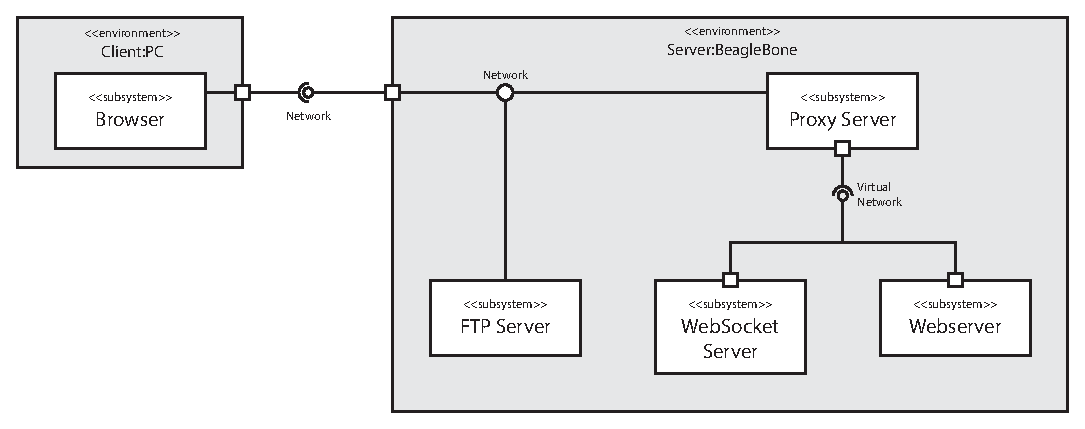
\includegraphics[width = 0.8\textwidth]{dokumentation/images/components.eps}
\caption{Funktionale Komponenten}
\label{fig:functionalComponents}
\end{figure}

Das Webinterface besteht aus drei funktionalen Teilen: auf der einen Seite der Webbrowser, der ausschließlich als Client dient und zum anderen aus dem WebSocket Server, der die Steuerung der \gls{gpio} erledigt und die Daten für die Konfiguration der Weboberfläche liefert und aus einem Webserver, der die Dokumente ausliefert. Um nach außen über einen einzigen Port zu kommunizieren, ist ein Proxy Server vorgelagert (Abb. \ref{fig:functionalComponents}), der den Datenverkehr an Hand des verwendeten Protokolls an den richtigen Server weiterleitet (Abb. \ref{fig:requestForwarding}).

\begin{figure}[ht]
\centering
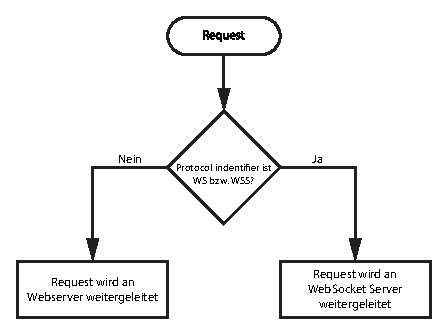
\includegraphics[width = 0.5\textwidth]{dokumentation/images/request.eps}
\caption{Verarbeitungschema eines Requests am Proxy Server}
\label{fig:requestForwarding}
\end{figure}

\noindent Die Auslagerung das Proxy Servers hat folgende Vorteile:

\begin{enumerate}
  \item Das \gls{ssl-offloading} wird von HAProxy automatisch vorgenommen.
  \item Der Webserver ist nicht direkt zu erreichen. D. h. eventuelle Einbruchsversuche über Fehler in der HTTP-Implemtierung von Lighttpd werden bereits im Proxy Server abgefangen, da ungültige HTTP-Header nicht weiterverarbeitet werden.
  \item Um die direkte Hardware-Steuerung zu übernehmen, muss der WebSocket Server mit root-Rechten betrieben werden. Da WebSocket Request nicht durch den Webserver geleitet werden, ist das System selbst bei einer Übernahme des Webservers weitegehend sicher. Zudem ist für den Betrieb keinerlei Kommunikation zwischen Webserver und WebSocket Server notwendig (Vgl. Abb. \ref{fig:pageloadSequence}).
  \item Das Projekt gestaltet sich übersichtlicher, da die einzelnen Komponenten über virtuelle Netzwerkverbindungen kommunizieren und somit leichter zu warten sind.   
  \item HAProxy ist im Feldeinsatz erprobt und kann angesichts der weiten Verbreitung auf namhaften Webseiten als ausreichend stabil angenommen werden \cite{kuehnast2014}, während die Proxy-Unterstützung in Lighttpd nur mäßig Dokumentiert ist.
\end{enumerate}


\section{Datenaustausch}
Der gesamte Datenaustausch des Interfaces läuft über die WebSocket-Verbindung ab. Dabei beinhaltet jede Message den Key \textit{type}, mit dem jeweils im Browser bzw. Websocket Server entschieden wird, wie weiter zu verfahren ist. Das \textit{parameters}-Objekt enthält alle weiteren Informationen (Abb. \ref{lst:requestMessage}).\\

\begin{figure}[ht]
\begin{lstlisting}
{
  type: "getPinMode",
  parameters: {
    pin: "P9_33"
  }
}
\end{lstlisting}
\caption{Auszug aus einer Request Message}
\label{lst:requestMessage}
\end{figure}

Um Antworten richtig zuordnen zu können, werden Rückgabewerte der Funktionen in einem \textit{response}-Objekt an die ursprüngliche Messsage angehängt. Alle Daten, die zu dieser Antwort geführt haben, sind dann noch vorhanden und können über einen Response Handler verarbeitet werden.\\

\begin{figure}[ht]
\begin{lstlisting}
{
  type: "getPinMode",
  parameters: {
    pin: "P9_33"
  },
  response: {
    pin: "P9_33",
    name: "AIN4"
  }
}
\end{lstlisting}
\caption{Auszug aus einer Response Message}
\label{lst:responseMessage}
\end{figure}

Durch diese Technik ist gewährleistet, dass das Interface immer aktiv bleibt und nicht durch eine langsame Netzweranbindung blockiert wird. Gleichzeitig werden asynchron eingehende Messages zeitlich unabhängig verarbeitet.

\section{Seitenaufruf}
Um die Systembelastung durch das Webinterface möglichst gering zu halten, wird die Webseite dynamisch über Templates in weiten Teilen erst im Browser generiert. Dabei wird der Nutzer zunächst via HTTP Digest Authentication autentifiziert. Ist diese erfolgreich, werden die Doumente der Webseite an den Browser ausgeliefert.\\

Abbildung \ref{fig:pageloadSequence} zeigt schematisch, wie die Initialisierung der Seite abläuft. Das Diagramm zeigt horizontal die vier beteiligten Entitäten und vertikal, ähnlich einem Sequenzdiagramm, den zeitlichen Ablauf. Antworten sind dabei immer asynchron Event-basiert. Gestrichelte Linien zeigen Antworten tieferliegender Schichten und Protokolle. Sie sind nicht Teil meiner Implementierung und sollen den Request/Response-Verlauf verdeutlichen. Die Authentifizierung ist im Webserver implementiert und Teil der Kommunikation zwischen Webbrowser und Webserver \cite{rfc7235}. Sie ist daher nicht im Diagramm explizit dargestellt.

\begin{figure}[ht]
  \centering
  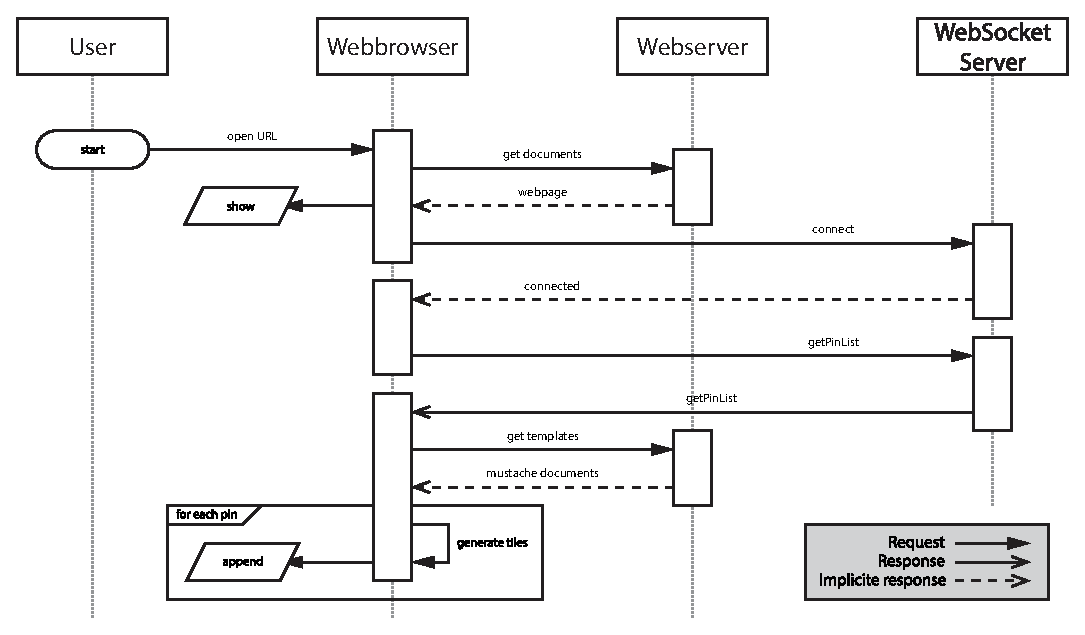
\includegraphics[width = \textwidth]{dokumentation/images/pageload.eps}
  \caption{Sequezieller Ablauf bei einem Seitenaufruf}
  \label{fig:pageloadSequence}
\end{figure}


\section{Interaktion}
Die Kommunikation mit dem WebSocket Server läuft vollständig asynchron ab. Es wird grundsätzlich keine direkte Antwort auf eine Anfrage erwartet um bei eventuell schlechter Netzwerverbindung nicht das Interface zu blockieren. Abbildung \ref{fig:interaction} zeigt diesen Vorgang exemplarisch.

\begin{figure}[ht]
  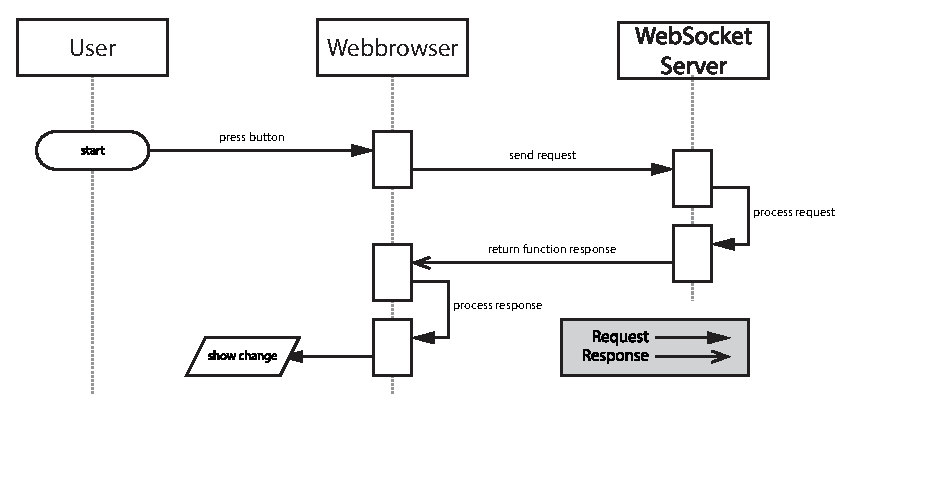
\includegraphics[width = \textwidth]{dokumentation/images/sendRequest.eps}
  \caption{Verarbeitung einer User-Interaktion}
  \label{fig:interaction}
\end{figure}


\section{WebSocket Server}
Der WebSocket Server ist vollständig in JavaScript/Node.js implementiert und modular aufgebaut. Alle notwendigen Dateien finden sich im Verzeichnes \textit{node/}.\\
Eine Besonderheit von JavaScript/Node.js ist es, dass sich Module grundsätzlich ähnlich wie ein Singleton Pattern verhalten. Dabei wird bei einem erneuten Aufruf von \textit{require()} keine neue Instanz erzeugt sondern Referenzen auf die erste übergeben.\\
So müssen bei asynchronen Funktionsaufrufen nicht alle benötigten Variablen übergeben werden und es wird sichergestellt, dass alle Funktionen auf denselben WebSocket zugreifen. Dies ist vor allem wichtig, da Intervalfunktionen, die via \textit{setInterval()} aufgerufen werden, keinen direkten Zugriff erlauben. Zudem sollen laufende Timer bei einem erneuten Besuch der Seite (oder eine reload) ihre Daten direkt wieder an den Browser senden.\\

Abbildung \ref{fig:wssDependencies} zeigt die Abhängigkeit zwischen den eizelnen Modulen. Im Kasten unter dem Modulnamen sind Abhängigkeiten dargestellt, die nicht Teil meiner Implementierung sind.

\begin{figure}[ht]
  \centering
  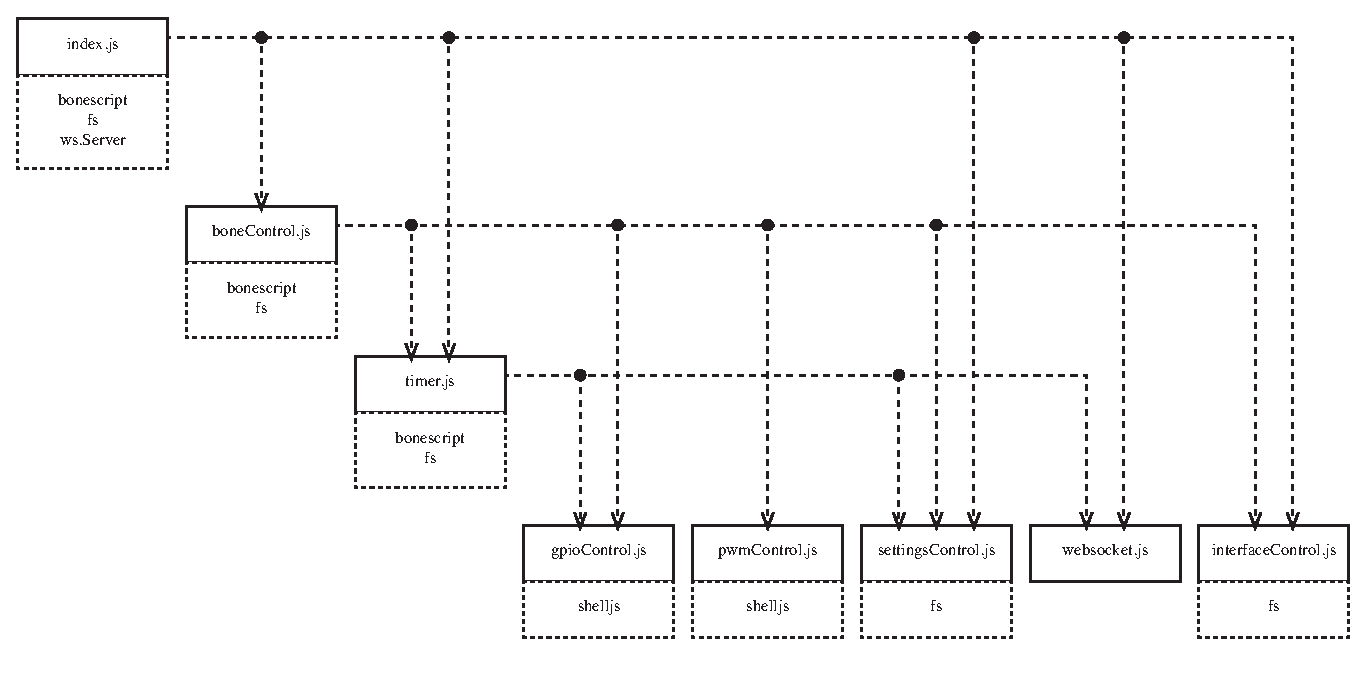
\includegraphics[width = \textwidth]{dokumentation/images/wssDependencies.eps}
  \caption{Abhängigkeiten der Module des WebSocket Server}
  \label{fig:wssDependencies}
\end{figure}

\subsubsection{index.js}
Die index.js stellt das Hauptdokument dar. Von hier aus wird der Server gestartet. Über den Aufruf \textit{require()} werden die Module des Servers geladen und die Event Listener für die WebSocket-Verbindung registriert.

Bei einem erfolgreichen Verbindungsaufbau wird der WebSocket im \textit{websocket}-Objekt referenziert und für alle anderen Module zugänglich gemacht.


\subsection{Models}

\subsubsection{interfaceControl.js}
\begin{wrapfigure}{r}{0.3\textwidth}
  \vspace{-16pt}
  \centering
  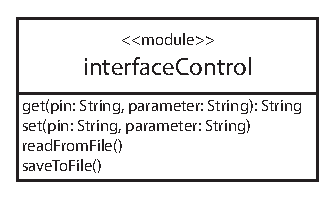
\includegraphics[width = 0.25\textwidth]{dokumentation/images/apiInterfaceControl.eps}
\end{wrapfigure}

Dieses Modul generiert bei Bedarf eine Liste der verfügbaren Pins und deren Typen Sowie deren letztmalige Interface-Konfiguration bezüglich aktiver und inaktiver Kacheln.\\

\noindent Zwei Dateien werden zur Generierung des interface-Objektes ausgelesen:

\begin{itemize}
  \item \textit{whitelist.json} enthält eine Liste der Pins mit Informationen über die Verwendbarkeit. Die Liste ist muss zur restlichen Software passen und wird vom Programm nicht verändert.
  \item \textit{interface.json} ist eine String-Version der letzten Interface-Konfiguration. Falls sie existiert, wird ein kombiniertes Objekt generiert um sicherzustellen, dass Informationen über das Interface nicht verloren gehen und eventuell zusätzliche Pins dennoch verfügbar sind.
\end{itemize}

Wenn die WebSocket-Verbindung geschlossen wird, wird das im Speicher befindliche Interface-Objekt in die Datei interface.json geschrieben und kann beim nächsten Aufruf der Seite erneut geladen werden.

\subsubsection{settingsControl.js}
\begin{wrapfigure}{r}{0.3\textwidth}
  \vspace{-16pt}
  \centering
  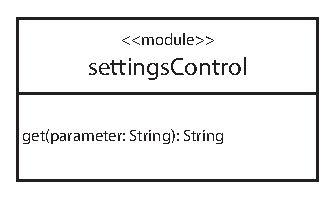
\includegraphics[width = 0.25\textwidth]{dokumentation/images/apiSettingsControl.eps}
\end{wrapfigure}

Das Modul \textit{settingsControl.js} liest die Einstellungsdateien ein und stellt diese programmweit zur Verfügung. Das Modul nutzt dafür die Datei \textit{settings-default.json}, in der alle Basiseinstellungen enthalten sind. Diese Einstellungen werden dann von denen in der Datei \textit{settings.json} überschrieben, sofern das Dokument vorhanden ist. Bei den beiden Dateien handelt es sich um \gls{json}-Files nach rfc6455 \cite{rfc6455}.

Es werden nur Parameter überschrieben, die sowohl in den Default-Einstellungen als auch in den eigenen vorhanden sind. So ist sicherggestellt, dass keine Pareter versehentlich ins System gelangen, die nicht vorgesehen sind. Desweiteren ist es möglich, nur die Einstellungen einzutragen, die geändert werden sollen.

\subsubsection{websocket.js}
\begin{wrapfigure}{r}{0.3\textwidth}
  \vspace{-16pt}
  \centering
  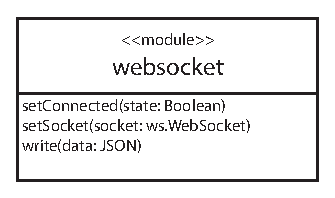
\includegraphics[width = 0.25\textwidth]{dokumentation/images/apiWebsocket.eps}
\end{wrapfigure}

Dieses Modul verwaltet die eigentliche WebSocket-Verbindung. Essenziell ist die Funktion \textit{write()}. Hierüber können die restlichen Module direk auf den Socket schreiben. Dabei wird intern geprüft ob der Socket noch offen ist. Wenn eine neue Verbindung hergestellt wurde, wird diese sofort wieder beschrieben.


\subsection{Controller-Module}
Ein weiterer Teil des WebSocket Servers besteht aus einer Reihe von Controller-Modulen, die verschiedene Steuerungen übernehmen.

\subsubsection{boneControl.js}
\begin{wrapfigure}{r}{0.3\textwidth}
  \vspace{-16pt}
  \centering
  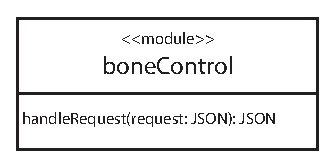
\includegraphics[width = 0.25\textwidth]{dokumentation/images/apiBoneControl.eps}
\end{wrapfigure}

Dieses Modul stellt den Kern der Hardware-Ansteuerung dar. Eingehende WebSocket Requests werden hier über \textit{type} identifiziert und abgearbeitet. Hierbei wird über eine Switch-Case-Anweisung entschieden was zu tun ist, Requests mit unbekanntem Typ werden mit einer Fehlermeldung im \textit{response}-Objekt an das Interface zurückgesendet (Abb. \ref{fig:wssResponseHandler}).

\begin{figure}[ht]
  \centering
  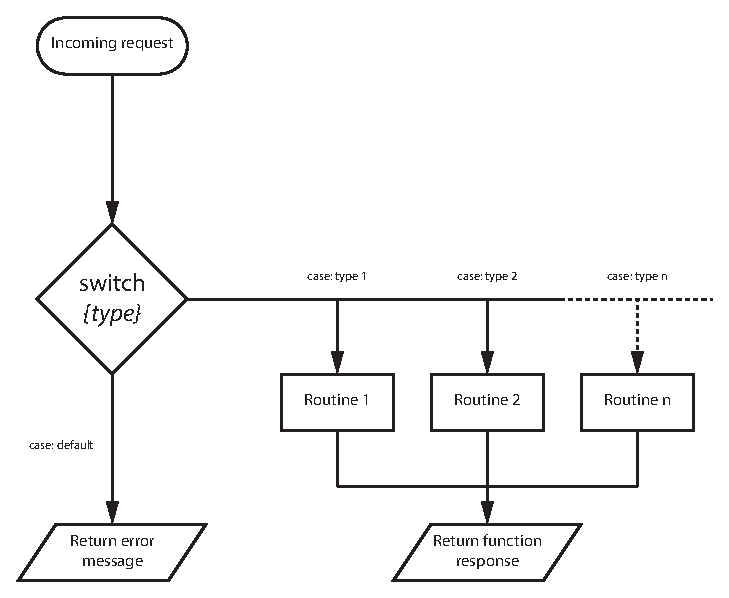
\includegraphics[width = 0.5\textwidth]{dokumentation/images/wssResponseHandler.eps}
  \caption{Schematische Arbeitsweise des Response Handlers}
  \label{fig:wssResponseHandler}
\end{figure}

Die API der \textit{bonescript} Library ist in dieser Liste weitgehend abgebildet. Daneben werden hier auch sämtliche Parameter für das Interface zusammengestellt und an den Browser gesendet.

\subsubsection{timer.js}
\begin{wrapfigure}{r}{0.3\textwidth}
  \vspace{-16pt}
  \centering
  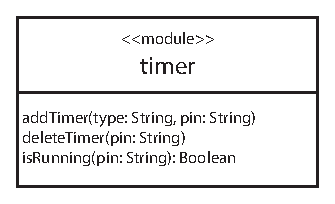
\includegraphics[width = 0.25\textwidth]{dokumentation/images/apiTimer.eps}
\end{wrapfigure}

Mit Hilfe dieses Moduls werden digitale und analoge Inputs verwaltet. Über eine Switch-Case-Anweisung wird geprüft ob es sich im einen analogen oder digitalen Input handelt und dann mit Hilfe von \textit{setInterval()} ein Timer gestartet, der zyklisch eine anonyme Callback Funktion aufruft. Das zeitliche Interval wird dem Settings Modul entnommen. Die Funktionen senden dann die Ergebnisse selbstständig an die Webseite. Fehlende Dateien, Links oder Ordner werden ebenfalls automatisch erstellt. Um den Timer wieder beenden zu können, wird die Funktion zusätzlich in einem lokalen Timer-Objekt registriert.

\paragraph{Digital Input} Um unnötiges Datenvolumen zu vermeiden prüft diese Funktion zunächst ob sich der Pin-Status gegenüber der letzten Abfrage geändert hat. Nur wenn das wenn sich der Wert unterscheidet, wird er an das Interface gesendet (Abb. \ref{fig:wssTimerDigital}).

\begin{figure}[H]
  \centering
  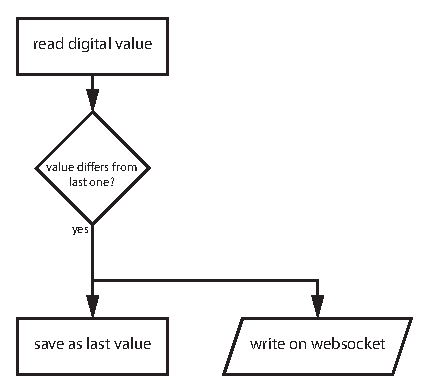
\includegraphics[width = 0.5\textwidth]{dokumentation/images/wssTimerDigital.eps}
  \caption{Anonyme \textit{digitalRead}-Funktion}
  \label{fig:wssTimerDigital}
\end{figure}

\paragraph{Analog Input} Die Funktion für den analogen Input produziert einen kontinuierlichen Datenstrom um ein fließendes Diagramm auf der Webseite zu realisieren und speichert diese Daten parallel in einer standardkonformen CSV-Datei \cite{rfc4180} (Abb. \ref{fig:wssTimerAnalog}).

\begin{figure}[H]
  \centering
  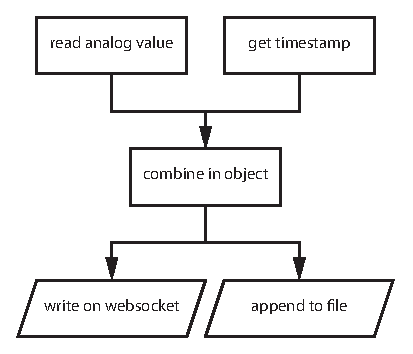
\includegraphics[width = 0.5\textwidth]{dokumentation/images/wssTimerAnalog.eps}
  \caption{Anonyme \textit{analogRead}-Funktion}
  \label{fig:wssTimerAnalog}
\end{figure}

\subsection{Bypass-Module}
Die bonescript Library weist in einigen Fällen Fehler oder fehlende Feature auf. Intern arbeitet die Bibliothek mit \gls{devicetree} Overlays allerdings ist es nicht möglich diese wieder zu entladen. Dies ist vor allem wichtig, wenn \gls{pwm}-Ausgänge bockiert wurden um einen zweiten synchronen Ausgang zu erhalten. Um diese Funktionalität zu implementieren habe ich zwei Bypass-Module geschrieben, die das digital I/O- und das PWM-Management übernehmen.

\subsubsection{gpioControl.js}
\begin{wrapfigure}{r}{0.3\textwidth}
  \vspace{-16pt}
  \centering
  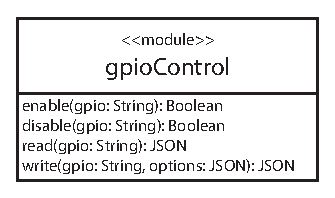
\includegraphics[width = 0.25\textwidth]{dokumentation/images/apiGPIOControl.eps}
\end{wrapfigure}

Dieses Modul steuert die digitalen I/O direkt über das Dateisystem. Dazu werden die in der bonescript Library hinterlegten Pin IDs genutzt.\\

Das Modul stellt Funktionen zum aktivieren und deaktivieren der \gls{gpio} zur verfügung, sowie zum Lesen und schreiben der Parameter. Parameter werden in Form eines \gls{json}-Objektes übergeben und sind jeweils optional.

\subsubsection{pwmControl.js}
\begin{wrapfigure}{r}{0.3\textwidth}
  \vspace{-16pt}
  \centering
  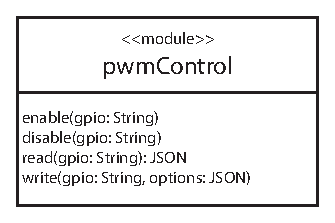
\includegraphics[width = 0.25\textwidth]{dokumentation/images/apiPWMControl.eps}
\end{wrapfigure}

Die API dieses Moduls verhält sich analog zu dem der \gls{gpio}. Intern werden Die Device Tree Overlays der bonescript Library verwendet. Diese werde per Filesystem über den \gls{capemgr} geladen.

\section{Website} Bei der Implementierung steht die Funktionalität im Fokus. Daher habe ich so viel wie möglich mit bereits existierenden Bibliotheken gearbeitet, um Design und Darstellung umzusetzen. Diese Bibliotheken basieren intern auf \gls{html}, \gls{css} und \gls{js}.\\
Die Website selbst besteht daher nur aus einem einzigen \gls{html}-Dokument, in dem die Basisstruktur der Seite definiert wird. In der index.html werden auch alle globalen Objekte wie die WebSocket-Verbindung und die Pin-Liste angelegt.\\

Bei einem Seitenaufruf werden zunächst die benötigten Bibliotheken beim Webserver angefordert und geladen. Das Event \textit{document.ready} stößt dann den Verbindungsaufbau zum WebSocket Server an. Ist die Verbindung hergestellt, wird das Event \textit{websocket.onopen} ausgelöst und die aktuelle Pin-Konfiguration vom Server angefordert.

Die weiteren Inhalte werden dynamisch via JavaScript und \gls{html}-Templates generiert.


\subsection{Skriptdokumente}
Die Funktionen für die Webseite sind analog zu den Modulen des WebSocket Servers aufgeteilt. Die Skriptdokumente der Webseite sind jeweils via \gls{json} mit einem Pseudo-Namespace versehen. Funktionen und Objekte sind dabei in einer \gls{json}-Struktur angelegt und können darüber abgerufen werden. Auch Sub Namespaces sind möglich um beispielsweise Hilfsfunktionen zu beherbergen (Abb. \ref{lst:pseudeNamespaceJS}).

\begin{figure}[ht]
  \begin{lstlisting}
  var bonescriptCtrl = {};
      bonescriptCtrl.util = {};
  \end{lstlisting}
  \caption{Pseudo-Namespace in JavaScript}
  \label{lst:pseudeNamespaceJS}
\end{figure}

Da es innerhalb des Browsers keine modulare Struktur wie im WebSocket Server gibt und um daher keinen falschen Eindruck zu erwecken, sind im folgenden sind alle Skriptdokumente alphabetisch zusammengestellt.

\begin{longtabu} to \textwidth {
  X[1]
  X[3]}
  \textbf{bonescriptCtrl.js} & Hier werden alle Funktionen zum Absetzen von Steuerbefehlen an den WebSocket Server definiert. Sowohl Befehle für die Hardware-Steuerung als auch für das Interface sind hinterlegt.\newline\\
  
  \textbf{diagramCtrl.js} & Enthält Funktionen um die Diagramme zu verwalten. Zum einen werden hierüber die Diagramme initialisiert und zum anderen Funktionen zum hizufügen neuer Wertepaare und zurücksetzten des Diagramms. Die Zeichengeschwindigkeit ist fest auf 25Hz gesetzt um die Systemlast möglicht gering zu halten.\newline\\

  \textbf{init.js} & Dieses Dokument liefert eine Funktion, \textit{init()}, in der der eigentliche Inhalt der Seite generiert wird. Sobald die Pin-Liste übermittelt wurde, arbeitet eine For-Each-Schleife jeden einzelnen Pin ab. Dabei werden via synchronem Ajax Request die Templates vom Webserver angefordert. Da die Dokumente zunächst im Cache des Browsers verbleiben, entsteht durch den häufigen Aufruf kein erhöhter Netzwerk-Traffic. Im Anschluss werden die Listener-Funktionen an Buttons, etc. angehängt.\newline\\

  \textbf{responseHandler.js} & Der Response Handler ist eine Sammlung von Funktionen um auf eingehende Messages zu reagieren. Zu jedem im WebSocket Server definierten \textit{type} gibt es hier eine entsprechende Funktion. Funktionsnamen sind identisch, damit die Fuktionen direkt aufgerufen werden können.\newline\\

  \textbf{util.js} & Dieses Dokument enthält einige Utility-Funktionen zur einfacheren Bedienung von Bootstrap.\newline\\

  \textbf{websocketCtrl.js} & Hier leigen die Listener-Funktionen für die WebSocket-Verbindung. Bei einem erfolgreichen Verbindungsaufbau wird der Buttom im Hautfenster verändert und der Init-Prozess angestoßen. Eingehende Messages werden in \gls{json}-Objekte übersetxzt und die entsprechende Funktion aus dem Response Handler aufgerufen.\newline\\
\end{longtabu}


\subsection{Bibliotheken}

\subsubsection{jQuery}
jQuery ist ein \gls{de-facto-Standard} zur \gls{dom}-Verwaltung. Diese Bibliothek ermöglicht objektähnliche Verwendung von \gls{html}-Elementen und stellt viele Rendering- und Animationsfunktionen zur Verfügung.\\

jQuery ist Vorraussetzung für alle weiteren Bibliotheken.


\subsubsection{Bootstrap \& jQuery-UI}
Bootstrap ist für die grafische Darstellung verantwortlich und wird dabei durch einzelne Funktionen aus jQuery-UI ergänzt. Hierbei ermöglicht das Framework das Kachelsystem, das zur Anordnung der Bedienelemente verwendet wird. Dieses System ermöglicht eine dynamische Darstellung, sodass deaktivierte Bedienelemente nicht einfach nur leere Felder hinterlassen. Die aktiven Felder werden vielmehr übersichtlich zusammen gerückt. Weiter generiert Bootstrap mit Hilfe von Themes alle Elemente wie Kopfleiste, Buttons oder Eingabemasken.\\


\subsubsection{Flot Diagrams}
Diese Bibliothek dient zum Zeichnen der Diagramme. Im Dokument wir hierfür nur ein Platzhalter eingetragen. Alles weitere wird von der Bibliothek geregelt. Um neue Punkte zu generieren, wird zunächst das Array, welches alle darzustellenden Tupel enthält, aktualitisiert und per Funktionsaufruf neu gerendert.


\subsubsection{Mustache.js}
Mustache.js ist eine JavaScript Implementierung des \href{http://mustache.github.io/}{Mustache Template System}. Mit diesem Tool lassen sich ohne großen Aufwand HTML-Templates schreiben, bei denen Variablen in doppelten geschweiften Klammern -- \{\{variable\}\} -- eingesetzt werden. Diese werden in der Laufzeit mittels \textit{Mustache.render()} zu einem gültigen HTML-String verarbeitet. Da sich die einzelnen Kacheln nur in der Pin-Bezeichnung unterscheiden, habe ich für jeden der drei Kacheltypen jeweils ein Template entworfen.
\chapter{Erweiterungsmöglichkeiten}
Im folgenden Kapitel werden weitere Möglichkeiten erläutert, durch die der Boneserver noch besser an bestehende Laborumgebungen angepasst und weiteres Potential des Konzeptes nutzbar gemacht werden kann.

\section{Zusätzliche Anpassungsoptionen}
Das Interface könnte durch zusätzliche Anpassungsoptionen erweitert werden. Eine Mög\-lich\-keit besteht darin, die einzelnen Kacheln mit individuellen Bezeichnungen zu versehen.

Der \textit{Interface Controller} kann dahingehend erweitert werden. Da im WebSocket Server die Pin-Konfiguration ohnehin in einer \gls{json}-Struktur gespeichet wird, können eventuelle Namen einfach hier gespeichert werden. Die Daten werden im Initialisierungsprozess der Seite automatisch an den Browser übertragen.

Im \textit{Init Script} kann die Weiterverarbeitung ähnlich dem Status der Kacheln implementiert werden (Abb. \ref{lst:fakeResponseMessage}).

\begin{figure}[H]
\begin{lstlisting}
for(pin in pins) {
  if (!pins[pin].active) {
    responseHandler.toggle({parameters: {pin: pin}, response: false});
  }
}
\end{lstlisting}
\caption{Fake response message, um geladene Kacheln zu verändern}
\label{lst:fakeResponseMessage}
\end{figure}


\section{Höher aufgelöste A/D-Wandlung}
Der maximale Takt der digitalen Inputs und der \gls{adc} ist durch die kleinste Zeiteinheit in JavaScript (1ms) vorgegeben. Denkbar wäre es, eine höher aufgelöste Taktung in einer separaten Software zu implementieren. In C/C++ könnte eine wesentlich höhere Ab\-tast\-rate erreicht werden. Diese Samples können dann zu mehreren als Antwort übertragen werden.\\

Der \textit{Diagram Controller} muss dahingehend erweitert werden, nicht nur einzelne Wertepaare zu verarbeiten (Abb. \ref{lst:insertTupel}), sondern oben beschriebene Frames. Je nach Abtastrate sollte auch über eine entsprechende Unterabtastung für die Anzeige nachgedacht werden.

\begin{figure}[H]
\begin{lstlisting}
diagramCtrl.util.addValue = function(pin, data) {
  diagramCtrl[pin]['data'].push(data);
}
\end{lstlisting}
\caption{Tupel in ein Diagramm einfügen}
\label{lst:insertTupel}
\end{figure}


\section{Alternative Steuerungsbibliothek -- octalbonescript}
Die Bibliothek \textit{octalbonescript}\footnote{https://github.com/theoctal/octalbonescript}, ein bonescript Fork, löst laut API verschiedene Probleme der Bonescript-Bibliothek. Sie könnte als Ersatz für die bisher verwendete Bonescript-Bibliothek genutzt werden. Dadurch würden auch die Module \textit{gpioControl.js} und \textit{pwmControl.js} nicht mehr nötig sein, da sie nur Bypassfunktionen für fehlerhafte Funktionen enthalten.


\section{Alternative Hardware}
Denkbar wäre eine Portierung des Boneservers auf eine andere Hardwareplattform. Die Voraussetzung hierfür ist ein Linux System mit einem Netzwerkzugang und entsprechendem Speicher.\\

Um auf einer anderen Hardware arbeiten zu können, ist eine passende Bibliothek wie die Bonescript-Bibliothek BeagleBone, nötig, um die Hardware zu steuern. Das Modul \textit{boneControl.js} regelt die gesamte Steuerung und muss dahingehend erweitert werden, dass die enthaltenen Fälle (Abb. \ref{lst:exampleCase}) passende Funktionen aus ihrer Bibliothek starten.

\begin{figure}[H]
\begin{lstlisting}
case 'analogRead':
  var pin = parameters.pin;

  response = bonescript[request.type](pin);
  break;
\end{lstlisting}
\caption{Beispiel-Case aus dem Modul \textit{boneControl.js}}
\label{lst:exampleCase}
\end{figure}


\section{Erweiterte Konfiguration in das Interface integrieren}
Die erweiterten Konfigurationsmöglichkeiten, die bisher aus Sicherheitsgründen nur über eine Konfigurationsdatei möglich waren, können in das Interface integriert werden. Das Authentifizierungssystem bietet hierfür die Möglichkeit, verschiedene Benutzer- und Ad\-mi\-ni\-stra\-tor-""Accounts einzurichten (vgl. Abb. \ref{lst:lighttpdhtdigest}). Dazu muss eine Administrationsseite geschrieben und in einem passenden Verzeichnis abgelegt werden. Die Zugriffsbeschränkungen können dann, wie oben beschrieben, separat für dieses Verzeichnis konfiguriert werden. Externe Laufwerke und USB-Sticks sollten dafür automatisch mit passenden Rechten eingebunden werden und in einem Menü auswählbar sein.


\section{Weitere GPIO}
Neben den bereits verfügbaren GPIO sind noch einige weitere vorhanden, die standardmäßig für den HDMI-Ausgang verwendet werden. Da das System primär per Fernzugriff verwaltet werden soll, kann der Anschluss deaktiviert werden. Diese GPIO können über die \textit{whitelist.json} freigegeben werden.
\chapter{Zusammenfassung}
Im Rahmen dieser Arbeit wurde von mir ein webbasiertes Steuersystem für Messanwendungen entwickelt und vorgestellt. Die Grundidee war, ein vereinfachtes, flexibles System anzubieten, das je nach Anwendungskontext individuell und ohne großen Aufwand angepasst werden kann. Hardware und Programmierung sollten hauptsächlich mit auf dem Markt vorhandenen Mitteln realisiert werden, um Entwicklungsaufwand und Kosten gering zu halten. Auch Rechenleistung und Energie sollten überschaubar bleiben. Von zentraler Bedeutung für das Messsystem allerdings ist, dass es über das Internet, abruf- und steuerbar ist.

Die Wahl der Hardware fiel auf den BeagleBone Black, weil bei ihm das Verhältnis zwischen Rechenleistung, Schnittstellenumfang und Preis gegenüber den Konkurrenzsystemen am günstigsten ist. Gleichzeitig ist der Prozessor eine aktive Produktlinie von Texas Instruments, einem namhaften Hersteller für Mikroprozessoren und es gibt bereits werksseitig eine Software-Bibliothek, die die rudimentäre Hardware-Steuerung übernimmt. Die Wahl des Betriebssystems fiel auf Arch Linux, ein minimales Linux System mit großen Anpassungsmöglichkeiten, da eine Eigenentwicklung den Rahmen dieser Arbeit bei weitem gesprengt hätte und Linux Systeme im Embedded-Bereich zurzeit einen De-Facto-Standard darstellen.\\

Da die Bibliothek zu steuerung der Hardware in JavaScript bzw. Node.js implemtiert ist, habe ich zunächst versucht, möglichst viel der benötigten Funktionalität via JavaScript umzusetzen. Größtes Problem dabei war, dass die meisten Webserver-Lösungen in Node.js im Zusammenhang mit dem BeagleBone viel zu langsam arbeiten. Zudem ist es sehr aufwändig,  die vollständige Funktionalität eines Webservers selbst zu implementieren und das gesamte System hätte mit root-Rechten laufen müssen, was bei Webservern aus Sicherheitsgründen grundsätzlich vermieden werden sollte. Hier wäre weiterer Aufwand durch gewissenhaftes Implementieren von Sicherheitsmechanismen entstanden. Dies war allerdings nicht Teil des Projektes. Aus diesen Gründen habe ich mich für ein mehrstufiges System entschieden, bei dem ein regulärer Webserver Dokumente ausliefert und ein zweites System sich ausschließlich mit der Verwaltung der GPIO beschäftigt.

Dabei stellte sich die Frage, in welcher Weise Steuerbefehle sinnvoll an den BeagleBone übertragen und Antworten bzw. Messdaten zurück erhalten werden könnten. Die Lösung dieses Problems fand sich in WebSockets und \gls{json}. Mit deren Hilfe ist es möglich Daten ohne großen Daten-Overhead strukturiert zu auszutauschen. Vorteilhaft ist ebenfalls, dass es bereits einige Implementierungen in Node.js in Form von Modulen gibt.\\

Das größte Problem wärend der Entwicklung bestand darin, dass die Bonescript-Bibliothek durch ihr frühes Entwicklungsstadium noch einige Fehler insbesondere in der Steuerung der Pulsbreitenmodulation aufweist. Lange Versuche diese Fehler zu beheben oder zu umgehen haben dazu geführt, dass ich die Funktionalität selbst in Modulform separat implementiert habe. Ziel ist es aber dennoch, diese Funktionaltät wieder in die Bibliothek zu verlagern, sobald die Probleme dort gelöst sind. 

Gegen Ende des Projektes bin ich auf eine alternartive Bibliothek gestoßen (\textit{octalbonescript}), die ihrer Beschreibung nach die API der Bonescript-Bibliothek vollständig implementiert, dabei allerdings wesentliche Fehler behebt. Im Rahmen dieser Arbeit blieb leider keine Zeit diese vielversprechende Alternative eingehend zu prüfen.\\

Das Ergebnis meiner Arbeit ist ein System, mit dem sich einfache Messumgebungen schnell erstellen lassen und das außer einer Netzwerkverbindung keiner weiteren Technik bedarf. Dabei ist es unerheblich, ob es sich bei dem Netzwerk um ein lokales Netzwerk, ein Intranet im Laborkoplex oder das Internet handelt. Da nur wichtig ist, dass das Netzwerk Betribssystemweit vorhanden ist, sind auch GSM- oder WLAN-Verbindungen kein Problem.

Diese Arbeit zeigt, dass es mit Hilfe von Webtechnologien wie HTML5 und WebSockets möglich ist Echtzeitmesssysteme zu realisieren, die existierende Hardware verwenden und dadurch wesentlich kostengünstiger sind als spezialisierte Systeme namhafter Hersteller.


\appendix
\part{Anhang}
\chapter{Betriebsanleitung}
\section{Hardware}
Dieses Handbuch ist für den \textbf{BeagleBone Black Revision A5C} (im Folgenden kurz als BeagleBone bezeichnet) geschrieben und getestet. Sofern nachfolgende oder vorangegangen Revisionen zu dieser kompatibel sind, sollte die Installation aber dennoch problemlos möglich sein.

\section{Installation}
Als Betriebssystem wird \href{http://archlinuxarm.org/}{Arch Linux ARM} verwendet, eine Portierung von Arch Linux für ARM-Prozessoren. Arch Linux ARM stellt auch ein spezielles package repository zur Verfügung.

\subsection{SD-Karte vorbereiten}
Auf der Homepage von Arch Linux ARM gibt es eine Installationsanleitung, die laufend aktualisiert wird. Die folgende Anleitung ist daher im Wesentlichen eine Übersetzung ausgehend von einem Linux als Host-System. Stattdessen kann auch die mitgelieferte {\AA}ngström Distribution verwendet werden, die mit dem BeagleBone ausgeliefert wird.

\paragraph{Voraussetzungen} sind die Softwarepakete \textit{dosfstools} und \textit{wget} sowie root-Rechte und eine Micro SD-Karte mit mindestens 2GB Speicherkapazität.

\begin{enumerate}

\item Finden Sie zunächst heraus, welcher Laufwerkspfad der vorgesehenen SD-Karte enspricht. Meist \textit{/dev/sd[a, b, ...]} oder \textit{/dev/mmcblk[0, 1, ...]}.

{\paragraph{\color{red} ACHTUNG} \textbf{\color{red} Überprüfen Sie Laufwerkspfade genau, bevor Sie mit der Installation beginnen, da sonst irreparable Schäden am Host-System auftreten können!}}

\item Starten Sie \emph{fdisk}, um die SD-Karte zu formatieren:

\begin{lstlisting}
fdisk /dev/sdX
\end{lstlisting}

\item Erstellen Sie eine neue Partitionstabelle und die nötigen Partitionen.\\
Dazu geben Sie nacheinander die folgenden Kommandos ein (jeweils mit \textit{enter} bestätigen):

\begin{longtabu} to \textwidth {
	X[1]
    X[3]}
\textbf{Kommando} & \textbf{Funktion}\\
o & Erzeugt eine neue Partitionstabelle\\
n, p, 1 & Erzeugt eine neue (n), primäre (p), erste (1) Partition\\
\textit{enter} & Bestätigt den Default-Wert für den ersten Sektor\\
+64M & +64M als letzten Sektor setzt die Partitionsgröße auf 64MByte\\
t, e & Ändert den Partitionstyp auf \textit{W95 FAT16 (LBA)}\\
a, 1 & Setzt das boot flag der ersten Partition (je nach \emph{fdisk}-Version wird die erste Partition automatisch ausgewählt, da nur eine zur Verfügung steht)\\
n, p, 2 & Erzeugt eine neue (n), primäre (p), zweite (2) Partition\\
2x \textit{enter} & Setzt die Default-Werte für den ersten und letzten Sektor der Partition\\
w & Schreibt Änderungen in die Partitonstabelle
\end{longtabu}

\item Formatieren der ersten Partition:

\begin{lstlisting}
mkfs.vfat -F 16 /dev/sdX1
\end{lstlisting}

\item Formatieren der zweiten Partition:

\begin{lstlisting}
mkfs.ext4 /dev/sdX2
\end{lstlisting}

\item Laden Sie den \textit{bootloader tarball} herunter und entpacken Sie ihn auf die erste Partition der SD-Karte:

\begin{lstlisting}
wget http://archlinuxarm.org/os/omap/BeagleBone-bootloader.tar.gz
mkdir boot
mount /dev/sdX1 boot
tar -xvf BeagleBone-bootloader.tar.gz -C boot
sync && umount boot
\end{lstlisting}

\item Laden Sie den \textit{rootfs tarball} herunter und entpacken Sie ihn auf die zweite Partition der SD-Karte (hierzu müssen Sie als \textit{root} eingeloggt sein, \emph{sudo} reicht in diesem Fall nicht):

\begin{lstlisting}
wget http://archlinuxarm.org/os/ArchLinuxARM-am33x-latest.tar.gz
mkdir root
mount /dev/sdX2 root
tar -xf ArchLinuxARM-am33x-latest.tar.gz -C root
sync && umount root
\end{lstlisting}

\item Stecken Sie die SD-Karte in den BeagleBone und halten Sie die Taste S2 gedrückt, um von der SD-Karte zu booten, während Sie die Power-Taste (S3) betätigen.\\
Wenn das System gestartet ist, können Sie sich auf der Kommandozeile oder via \emph{ssh} einloggen.\\

Benutzernahme/Passwort lautet \textbf{root/root}.

\end{enumerate}

Aus Sicherheitsgründen sollten Sie nach dem Systemstart als erstes das root-Passwort ändern:

\begin{lstlisting}
passwd root
\end{lstlisting}

Da man sich, außer zu Wartungszwecken, nicht am System anmelden muss, kann auf die Erstellung eines regulären Benutzers verzichtet werden.


\subsection{Installation im internen Speicher}

\paragraph{Hinweis} Der BeagleBone hat zwar eine eingebaute Uhr allerdings keine Batterie. Nach einem Neustart kann es daher passieren, dass die interne Uhr auf den Default-Wert zurück gesetzt wird. Überprüfen Sie mittels \emph{date} die aktuelle Systemzeit und aktualisieren diese gegebenenfalls via \texttt{ntpdate -u pool.ntp.org}

\begin{enumerate}
\item Um Arch Linux direkt auf der eMMC zu installieren, aktualisieren Sie zunächst das eben gestartete System und installieren die Pakete \emph{wget}, \emph{dosfstools} und \emph{ntp}.

\begin{lstlisting}
pacman -Syu wget dosfstools ntp
\end{lstlisting}

Das Paket \emph{ntp} stellt hierbei das Programm \emph{ntpdate} zur Verfügung (s. O.).

\item Der interne Speicher ist bereits korrekt partitioniert, folgen Sie daher nur den Schritten 4 bis 7. Die Partionen sind \textit{mmcblk1p1} bzw. \textit{mmcblk1p2} (s. O.).

\item Fahren Sie das System herunter und warten Sie bis alle LEDs erloschen sind.

\item Entfernen Sie die SD-Karte und starten das System erneut.
\end{enumerate}


\subsection{boneserver installieren}

\paragraph{Repository klonen}
\textit{boneserver} ist via \href{https://github.com/XMrVertigoX}{GitHub}\footnote{https://github.com/XMrVertigoX} verfügbar. Führen Sie dazu zunächt ein Systemupdate durch, um alle Pakete auf den neusten Stand zu bringen und installieren Sie das Paket \emph{git}. Anschließend klonen Sie das Repository nach \texttt{/opt}.

\begin{lstlisting}
pacman -Syu git
git -C /opt clone https://github.com/XMrVertigoX/boneserver.git
\end{lstlisting}

\paragraph{Installationsskript ausführen} Im root-Verzeichnis des Repositories befindet sich ein Skript, welches die weitere Installtaion übernimmt. Wechseln Sie dazu in das Verzeichniss und führen das Installationsskript aus.

\begin{lstlisting}
cd /opt/boneserver
./install.sh
\end{lstlisting}

Hierbei werden alle erforderlichen Pakete und Module installiert, die Konfigurationsdateien verlinkt sowie die Daemons installiert und gestartet.\\

Wenn das Skript fehlerfrei durchgelaufen ist, wird der BeagleBone automatisch neu gestartet und die Installation ist abgeschlossen.

\section{Betrieb}
Für die Verwendung des Webinterface wird eine Netzwerkverbindung zum BeagleBone und ein Webbrowser\footnote{Das Webinterface verwendet \emph{JQuery} in der Version 2.1.1, aktuelle webbrowser sollten hier keine Probleme bereiten. Ansonsten kann die Homepage von JQuery konsultiert werden: \url{http://jquery.com/browser-support/}} mit aktiviertem JavaScript vorausgesetzt.


\subsection{Netzwerkverbindung herstellen}

\paragraph{Hinweis:} Die Standardkonfiguration des BeagleBone sieht den Betrieb mit einem DHCP-Server vor. Sollte dies nicht gewünscht oder möglich sein, kann über die üblichen Wege eine statische IP eingestellt werden. Anleitungen hierzu findet man im Internet.\\

Steht ein DNS-Server zur Verfügung, kann der BeagleBone über seinen Hostname erreicht werden, standardmäßig \textit{boneserver}. Ansonsten finden Sie zunächst heraus, welche IP dem BeagleBone zugewiesen wurde. Hierfür kann entweder die Routing-Tabelle des DHCP-Servers konsultiert werden oder in der Kommandozeile via \emph{ip} die aktuelle Addresse der einzelnen Netzwerkadapter abgerufen werden \mbox{(Abb. \ref{fig:getBeagleBoneIP})}.

\begin{figure}[ht]
	\centering
	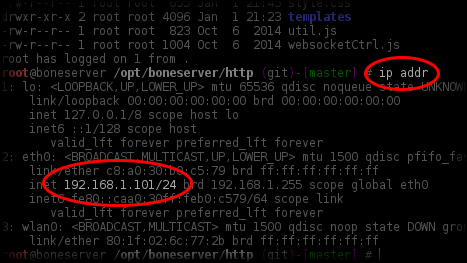
\includegraphics[width=0.7\textwidth]{betriebsanleitung/images/getBeagleBoneIP.png}
	\caption{IP des BeagleBone abrufen}
	\label{fig:getBeagleBoneIP}
\end{figure}


\subsection{Webinterface aufrufen}
Das Webinterface kann einfach über DNS-Namen oder die IP im Webbrowser aufgerufen werden. Ist die Verbindung hergestellt, wird dies durch einen grünen Haken rechts in der Titelleiste angezeigt \mbox{(Abb. \ref{fig:mainWindowConnected})} und die Steuerelemente werden generiert.
Sollte die Verbindung einmal unterbrochen werden, wechselt dieser Haken in ein rotes Kreuz. In diesem Fall kann die Seite neu geladen werden, eventuelle Konfigurationen bleiben erhalten.

\paragraph{Passwortschutz} Um unbefugten Zugriff zu verhindern ist das Webinterface passwortgeschützt. Wenn Sie dieses Passwort änderen möchten, generieren Sie zunächst einen neuen Datensatz z. B. mit dem \href{http://jesin.tk/tools/htdigest-generator-tool/}{\textit{htdigest Generator Tool}}\footnote{ \url{http://jesin.tk/tools/htdigest-generator-tool/}} und tragen die Zugangsdaten in die Datei \textit{config/lighttpd/lighttpd.user} ein. Die Default Login-Daten sind \textbf{admin/AgG7KgW4}

\begin{figure}[ht] 
	\centering
	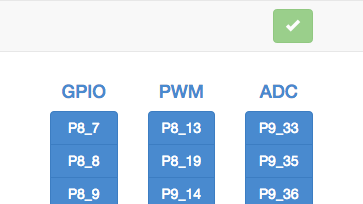
\includegraphics[]{betriebsanleitung/images/mainWindowConnected.png}
	\caption{Webinterface verbunden}
	\label{fig:mainWindowConnected}
\end{figure}

\paragraph{Hinweis} Das Webinterface kann immer nur von einem Fenster aus aufgerufen werden. Es kann daher passieren, dass bei einem schnellen Fensterwechsel oder Neuladen der Seite die Verbindung nicht sofort hergestellt wird. In dem Fall einfach ein paar (Milli-)Sekunden warten, bis die Verbindung wieder frei ist.


\subsection{Bedienelemente}
Wie in \mbox{Abbildung \ref{fig:webinterface}} gezeigt hat die Weboberfläche des boneserver drei Anzeigegruppen:

\begin{itemize}
\item[\textbf{1}] \textbf{Verbindungsanzeige}\\
zeigt grün, wenn die Steuereinheit verbunden ist und rot, wenn die Verbindung unterbrochen ist (vgl. Abb. \ref{fig:mainWindowConnected}).
\item[\textbf{2}] \textbf{Bedienfelder} für digitale I/O, PWM und AIN\\
Hier findet die tatsächliche Bedienung der GPIO statt. Es gibt drei Sektionen jeweils für digitale I/O, PWM und AIN. Die Bedienung der verschiedenen Kacheln wird weiter unten beschrieben.
\item[\textbf{3}] \textbf{Anzeigenschalter} für die einzelnen Pins\\
Hier können einzelne Kacheln ein- bzw. ausgeblendet werden, um die Oberfläche übersichtlicher zu gestalten und an die Arbeitsumgebung anzupassen. Diese Funktion dient ausschließlich der Übersicht, eine ausgeblendete Kachel bleibt weiterhin aktiv und kann jederzeit wieder eingeblendet werden. Diese Einstellungen bleiben auch nach einem Neustart erhalten.
\end{itemize}

\begin{figure}[ht] 
	\centering
	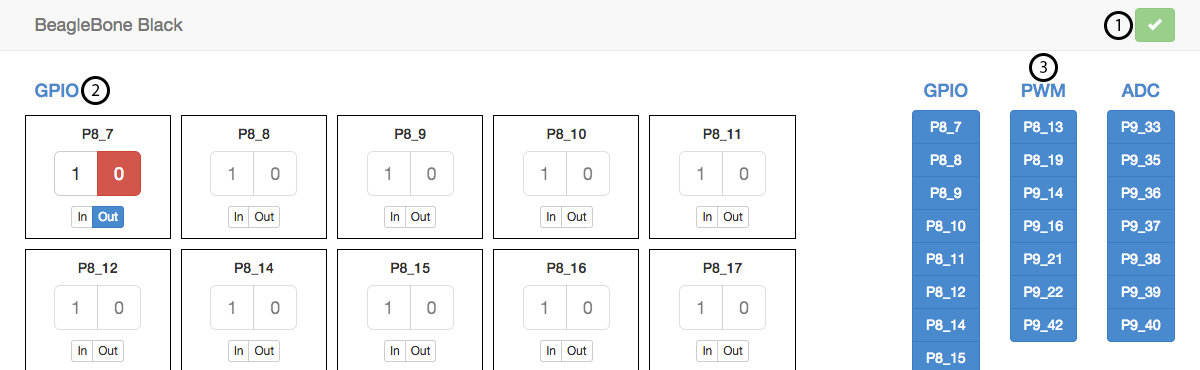
\includegraphics[width=1.0\textwidth]{betriebsanleitung/images/controlElements.png}
	\caption{Weboberfläche}
	\label{fig:webinterface}
\end{figure}

\subsubsection{Digitale In- und Outputs}
Die Konfigurationskachel \mbox{(Abb. \ref{fig:mainWindowGPIODisabled})} für digitale I/O besteht aus zwei Schaltern: Betriebsrichtung und logic level.

\paragraph{Betriebsrichtung} Jeder digitale I/O kann entweder als Input oder als Output konfiguriert werden. Dazu kann über den Wahlschalter \textbf{In/Out} jederzeit das Gewüschte ausgewählt werden.

\paragraph{logic level} Wenn der GPIO als Output konfiguriert ist, kann hier mittels der beiden Schaltflächen, \textbf{1} und \textbf{0}, ein logisches high und ein logisches low eingestellt werden. Ist der GPIO als Input konfiguriert, ist diese Schaltfläche deaktiviert und zeigt stattdessen den Status der Leitung an. Die GPIO sind mit einem internen Pulldown-Widerstand beschaltet.

\begin{figure}[ht] 
	\centering
	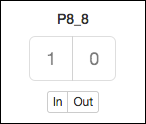
\includegraphics[]{betriebsanleitung/images/mainWindowGPIODisabled.png}
	\caption{Deaktivierte GPIO-Kachel}
	\label{fig:mainWindowGPIODisabled}
\end{figure}


\subsubsection{Pulsbreitenmodulation (PWM)}
Mit Hilfe der PWM-Kacheln \mbox{(Abb. \ref{fig:mainWindowPWMDisabled})} werden die GPIO konfiguriert, über die eine Pulsbreitenmodulation möglich ist.\\

Der BeagleBone stellt insgesamt sieben PWM-Ausgänge mit insgesamt vier Timern zur Verfügung. Dabei teilen sich jeweils die Pinne P8\_13/19, P9\_14/16 und P9\_21/22 einen Timer. P9\_42 hat einen exklusiven Timer. Die Ausgänge mit einem gemeinsamen Timer haben dementsprechend immer dieselbe Frequenz und laufen absolut synchron.\\

Über die Buttons \textbf{Enable} und \textbf{Disable} kann der jeweilige Ausgang aktiviert bzw. deaktiviert werden. Wenn ein PWM-Ausgang deaktiviert wird, werden alle Einstellungen bezüglich Frequenz und Pulsbreite gelöscht!

\paragraph{Periodendauer} Über das Eingabefeld \textbf{Period} wird die Periodendauer in Nanosekunden (ns) eingestellt. Kleinster Wert ist hier 1 ns ($\hat{=}$ 1GHz) und der größte $10^9$ ns (= 1s $\hat{=}$ 1Hz).

\paragraph{Pulsbreite} Über das Eingabefeld \textbf{Duty} wird die Pulsbreite zwischen 0 und 1 eingestellt. Hier wird intern ebenfalls mit Nanosekunden gearbeitet, daher kann der tatsächliche Wert zusätzliche Nachkommastellen bekommen.

\begin{figure}[ht] 
	\centering
	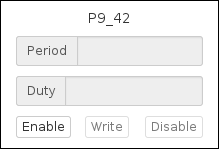
\includegraphics[]{betriebsanleitung/images/mainWindowPWMDisabled.png}
	\caption{Deaktivierte PWM-Kachel}
	\label{fig:mainWindowPWMDisabled}
\end{figure}

Mit \textbf{Write} werden die Parameter abgesendet.

\paragraph{Hinweis} Der Linux Kernel arbeitet intern mit ganzen Nanosekunden, daher ist die Genauigkeit der Pulsbreite von der Höhe der Periodendauer anhängig.

\paragraph{Bug:} Wenn beide Ausgänge eines PWM-Generators aktiviert sind, lässt sich die Frequenz bei keinem der beiden ändern. Wenn bei einem der beiden PWMs die Frequenz zunächst geändert wurde, kann der zweite Ausgang nicht verwendet werden. Dies ist ein Problem der im Hintergrund verwendeten device tree overlays und wird in nachfolgenden Versionen der Bibliothek behoben.


\subsubsection{Analoge Inputs}
Mit diesen Kacheln \mbox{(Abb. \ref{fig:mainWindowADC})} werden die Analog/Digital-Converter gesteuert und die Eingangswerte in einem Echtzeitdiagramm angezeigt.\\

Mit den Tasten \textbf{Start} und \textbf{Stop} wird die Aufzeichnung gestartet bzw. gestoppt. Parallel zur Anzeige werden die Messdaten aufgezeichnet. Über \textbf{Download} können sie als CSV-Datei heruntergeladen werden.\\

Die Taste \textbf{Delete} löscht die zu diesem Eingang gespeicherte Messreihe um Speicherplatz frei zu machen.

\paragraph{\color{red} ACHTUNG} \textbf{\color{red} Laden sie Messreihen immer herunter, bevor Sie sie löschen, die Messdaten sind sonst unwiederbringlich verloren!}

\begin{figure}[ht] 
	\centering
	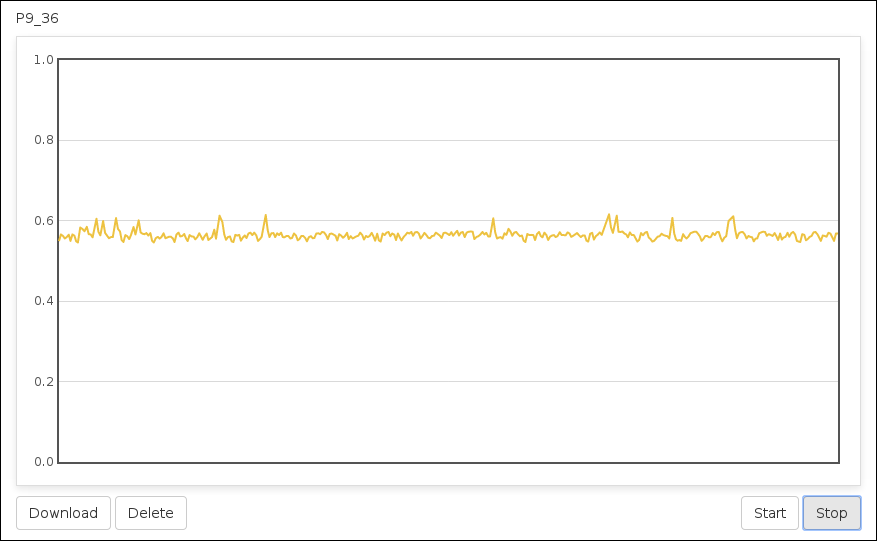
\includegraphics[width=0.9\textwidth]{betriebsanleitung/images/mainWindowAIN.png}
	\caption{ADC-Kachel}
	\label{fig:mainWindowADC}
\end{figure}


\subsection{Erweiterte Einstellungen}
Zusätzlich gibt es die Möglichkeit, über die Datei \textit{settings.json} im root-Verzeichnis des boneserver weitere Einstellungen vorzunehmen. Ist keine solche Datei vorhanden, wird die mitgelieferte \textit{settings-default.json} verwendet. Die Parameter überschreiben die Default-Werte, es müssen daher nur abweichende Werte eingetragen werden.\\

Die Datei ist eine JSON\footnote{JavaScript Object Notation (JSON) ist in der RFC 7159 beschrieben}-Datei in der folgende Parameter eingestellt werden können:\\

\begin{longtabu} to \textwidth {X[1] X[3]}
    
  \textbf{host} & IP des WebSocket Servers\newline
  Dieser Wert sollte nicht verändert werden, da sonst der WebSocket Server möglicherweise nicht mehr über das Webinterface erreichbar ist.\newline
  \textit{default: localhost}\\
  \textbf{port} & Netzwerk-Port des WebSocket Servers\newline
  Dieser Wert sollte nicht verändert werden, da der WebSocket Server sonst nicht mehr über das Webinterface erreichbar ist.\newline
  \textit{default: 8081}\\
  \textbf{gpioSampleRate} & Abtastrate der digitalen Inputs in Millisekunden\newline
  Angegeben wird die Zeit zwischen den Abfragen. Dieser Wert kann erhöht werden um die System- und Netzwerklast zu verringern.\newline
  \textit{default: 100}\\
  \textbf{adcSampleRate} & Abtastrate der analogen Inputs in Millisekunden\newline
  Angegeben wird die Zeit zwischen den Abfragen. Dieser Wert kann erhöht werden, um die System- und Netzwerklast sowie um die Menge der erhobenen Messwerte zu verringern. Dies ermöglicht bei gleichem Speicherplatz längere Messreihen.\newline
  \textit{default: 10}\\
  \textbf{dataLocation} & Speicherpfad für die Messdaten der ADC\newline
  Hier kann ein alternativer Pfad zur Speicherung der Messdaten eintragen werden. Es können auch externe Speicherorte wie z. B. USB-Sticks, USB-Festplatten oder Netzlaufwerke verwendet werden.\newline
  \textit{default: ./data}
\end{longtabu}

\paragraph{Hinweis} Die Datei \textit{settings-default.json} sollte nicht verändert werden, da sonst nicht ohne weiteres ein Update durchgfeührt werden kann.

\section{Wartung}
Als Wartungssystem wird die oben erstellte SD-Karte verwendet. Dazu starten Sie den BeagleBone von der SD-Karte und führen die oben beschriebenen Installationsschritte aus.\\

Die Paketverwaltung unter Arch Linux heißt \emph{pacman}, über sie können neue Pakete aus den Repositories installiert bzw. aktualisiert werden.\\
Ein kurzer Auszug aus der man-page zu den hier verwendeten Parametern:\\

Synopsis: \texttt{pacman <operation> [options] [targets]}\\

\begin{longtabu} to \textwidth {X[1] X[4]}

\textbf{Parameter} & \textbf{Beschreibung}\\
\textit{Operations}\\
-S, -\--sync & Synchronize packages. Packages are installed directly from the ftp servers, including all dependencies required to run the packages.\\

\textit{Sync Options}\\
-c, -\--clean & Remove packages that are no longer installed from the cache as well as currently unused sync databases to free up disk space.\\
-u, -\--sysupgrade & Upgrades all packages that are out of date.\\
-y, -\--refresh & Download a fresh copy of the master package list from the server(s) [...]. This should typically be used each time you use \textit{-u} or \textit{-\--sysupgrade}.\\
\end{longtabu}


\subsection{Backup}
Da der interne Speicher des BeagleBone \glqq nur\grqq ~2GB beträgt, kann ohne größerem Zeitaufwand ein komplettes Speicherabbild erstellt werden. Dies hat den Vorteil, dass es beim Einspielen von Backups keine Kompatibilitätsprobleme auftreten können.

Im Ordner \glqq scripts\grqq ~sind zwei shell-Skripte, die diesen Vorgang vereinfachen: \textit{backup.sh} und \textit{restore.sh}. Dabei wird das Image automatisch mit \emph{gzip} komprimiert, um Speicherplatz zu sparen. Das restore-Skript verwendet diese Dateien, um das Speicherabbild wieder auf den BeagleBone zu kopieren.\\

Sollte die SD-Karte nicht genügend Speicherplatz zur Verfügung stellen, kann ein USB-Stick verwendet werden. Dazu einfach das USB-Laufwerk einhängen\footnote{Anleitungen hierzu gibt es in ausreichender Zahl im Internet} und das entsprechende Verzeichnis als Zielverzeichnis angeben.

\begin{lstlisting}
backup.sh [Zielverzeichnis]
\end{lstlisting}

Das Zielverzeichnis ist dabei optional. Wenn kein Parameter übergeben wird, erstellt das Skript automatisch eine Datei in der Form \textit{backup-[timestamp].img.gz} im aktuellen Verzeichnis.

\begin{lstlisting}
restore.sh <Quelldatei>
\end{lstlisting}

Die Quelldatei ist hier Vorraussetzung.

\paragraph{Hinweis} Die Skripte verwenden intern \emph{dd}, um eine bitweise Kopie der eMMC des BeagleBone anzufertigen. Zudem ist die Quelle bzw. das Ziel immer \textit{/dev/mmcblk1}. Daher sollten diese Skripte nur von der SD-Karte aus verwendet werden.


\subsection{System aktualisieren}
Arch Linux verwendet die Rolling-Release-Technik, ein System, bei dem es keine großen Upgrades des gesamten Betriebssystems gibt, sondern die Softwarepakete einzeln laufend aktualisiert werden.\\
Trotz umfangreicher Tests der Pakete kann es zu Inkompatibilitäten kommen. Dies ist wahrscheinlicher, je mehr Pakete gleichzeitig aktualisiert werden. Daher sollte, gerade wenn das System nur selten aktualisiert wird, vorher ein vollständiges Backup angelegt werden (s. o.).\\

Das System kann jederzeit via \emph{pacman} aktualisiert werden:

\begin{lstlisting}
pacman -Syu
\end{lstlisting}


\subsection{boneserver aktualisieren}
Um die boneserver-Software zu aktualisieren, aktualisieren Sie zunächt Ihre Kopie des git Repositories und führen das Installationsskript erneut aus. Pakete, die bereits installiert sind, werden dabei nicht erneut installiert.

\begin{lstlisting}
cd /opt/boneserver
git pull
./install.sh
\end{lstlisting}


\subsection{System bereinigen}
\emph{pacman} speichert bei jeder Aktualisierung die alten Pakete, um jederzeit auf frühere Versionen zurückgreifen zu können. Je nach Häufigkeit der Aktualisierung und gemessen an der Kapazität der eMMC, kann der Speicher schnell knapp werden. Daher können alte Pakete via pacman in zwei Stufen gelöscht werden:

\begin{lstlisting}
pacman -Sc 
\end{lstlisting}

Löscht alle Paketversionen nicht mehr installierter Pakete und

\begin{lstlisting}
pacman -Scc
\end{lstlisting}

löscht sämtliche nicht verwendeten Pakete.


\chapter{Tabellen}

\begin{longtabu} to \textwidth {
  X[1]
  X[4]}
  \textbf{Paketname} & \textbf{Kurzbeschreibung}\\
  base-devel & Enthält die benötigten Entwicklertools\\
  python2 & Python in der Version 2. Wird für den Node Package Manager benötigt.\\
  lighttpd  & Der Webserver (siehe Abschnitt \ref{subsec:Lighttpd}).\\
  vsftpd & Ein FTP-Server. Wird verwendet um Messdaten ohne Webinterface automatisch abzurufen (siehe Abschnitt \ref{subsec:vsftpd}).\\
  linux-headers-am33x-legacy & Linux Header Files. Werden benötigt um Device Tree Overlays zu kompilieren.\\
  nodejs & JavaScript Engine (Siehe Abschnitt \ref{subsec:Node.js}).\\
  wget & Freies Kommandozeilenprogram um Dateien aus dem Internet herunterladen zu können.\\
  zsh & Alternative Kommandozeile (Z-Shell). Hohe Anpassungsmöglichkeiten.\\
  grml-zsh-config & Konfigurationsdateien für zsh.\\
  wpa\_supplicant & Unterstützung für WPA-Verschlüsselte WLAN.\\
  pv & Pipe Viewer. Wird von den Skripten \textit{backup.sh} und \textit{restpre.sh} verwendet um Speicherabbilder des BeagleBone zu erstellen.\\
  dtc-git-patched-20130410-1 & Device Tree Compiler mit \textit{dynamic link}-Patch. Wird von der bonescript library benötigt.\\
  haproxy-1.5.3-1 & Der Proxy-Server (siehe Abschnitt \ref{subsec:HAProxy}).\\
  
  \caption{Liste der benötigten Zusatzpakete}\\
  \label{tab:additionalPackages}\\
\end{longtabu}

\printglossary[title = {Glossar}]
\bibliography{literature.bib}
\addchap{Eidesstattliche Erklärung}

\noindent Ich versichere hiermit, die vorgelegte Arbeit in dem gemeldeten Zeitraum ohne fremde Hilfe verfasst und mich keiner anderen als der angegebenen Hilfsmittel und Quellen bedient zu haben.

\vfill

\noindent Köln, den \today \\[1cm]

\noindent (Caspar Friedrich)


\end{document}